\documentclass{beamer}
% 
% Choose how your presentation looks.
% 
% For more themes, color themes and font themes, see:
% http://deic.uab.es/~iblanes/beamer_gallery/index_by_theme.html
% 
\mode<presentation>
{
  \usetheme{Berlin}      % or try Darmstadt, Madrid, Warsaw, ...
  \usecolortheme{default} % or try albatross, beaver, crane, ...
  \usefonttheme{default}  % or try serif, structurebold, ...
  \setbeamertemplate{navigation symbols}{}
  \setbeamertemplate{caption}[numbered]
} 

\usepackage{default}
\usepackage{biblatex}
\usepackage{graphicx}
\setbeamerfont{caption}{size=\scriptsize}
\setbeamerfont{footnote}{size=\tiny}

\graphicspath{{figures/}}
\bibliography{references}

\title{Selecting Scenarios in Temporal Ensembles}
\author{Guilherme Gon\c{c}alves Schardong}
\date{\today}

\begin{document}
	
\begin{frame}
  \titlepage
\end{frame}

\begin{frame}{Outline}
  \tableofcontents
\end{frame}

\section{Introduction}
\begin{frame}
  \tableofcontents[currentsection]
\end{frame}

\begin{frame}{Introduction}
  \begin{itemize}
    \item Increased use of ensemble based methods;
    \item Difficulty to ``sift'' through this data and discover useful knowledge;
    \item Need of approaches to make the amount of data more tractable;
  \end{itemize}
\end{frame}

\begin{frame}{Research Questions}
  \begin{itemize}
    \item Given an ensemble of time series, how can we select a representative subset of them, such that analysis tasks done with the subset can be extended to the original set?
    \item How can we evaluate the quality of the selection approach? Is there a way to evaluate it in the first place?
  \end{itemize}
\end{frame}

\begin{frame}{Objectives}
  \begin{itemize}
    \item Develop an approach to select representative time series from an ensemble;
    \item Develop a visualization tool to help analyze the adherence of the ensemble's series compared to a reference series.
  \end{itemize}
\end{frame}

\section{Literature Review}
\begin{frame}
  \tableofcontents[currentsection]
\end{frame}

\begin{frame}{MinMax Approach}
  \begin{itemize}
    \item Sarma et al. \footfullcite{selection-sarma:2013} stated that most oil reservoir selection approaches relied on clustering algorithms and manual approaches;
    \item They stated that these approaches lead to suboptimal selections;
    \item They approached this problem from an optimization point of view;
    \item The approach developed was called MinMax and was able to select models representative in multiple properties and with a high coverage of the simulation's input uncertainty space.
  \end{itemize}
\end{frame}

\begin{frame}{Meira's Approach}
  \begin{itemize}
    \item Meira et al. \footfullcite{meira:2016} proposed the selection of the P$_{50}$ representative models of oil reservoir ensembles;
    \item They employed the MinMax approach proposed by Sarma et al. and fit it into a decision analysis methodology proposed by Schiozer et al. \footfullcite{schiozer:2015};
    \item Aims to minimize a multi-objecive cost function composed by a risk curve factor, and attribute-level coverage factor and a weighted cross plot spread factor;
    \item Selects high quality models without pessimistic or optimistic biases.
  \end{itemize}
\end{frame}

\section{Case Study: UNISIM-I}
\begin{frame}
  \tableofcontents[currentsection]
\end{frame}

\begin{frame}{Ensemble Description}
  \begin{itemize}
    \item UNISIM-I: High quality synthetic model for testing reservoir management methods and algorithms;
    \item Base model contains 30 years worth of data: 20 years of historic data (sampled on a monthly basis) and 10 years of forecast data (sampled every 6 months);
    \item Model contains 25 wells: 14 producers and 11 injectors;
    \item Our analysis was focused on the oil production of the 14 producer wells.
  \end{itemize}
\end{frame}

\subsection{Score-based Selection}
\begin{frame}{Score-based Selection}
  \begin{itemize}
    \item A ranking is done by ordering the distance of each time series to a reference curve at each time step;
    \item A score is attributed to each possible ranking (closer series will rank better, thus their score will be higher);
    \item A weight factor can be assigned to each time step, so that time series with a better ranking at those time steps will score higher;
    \item The $k$ highest scored series are then selected as possible representatives;
  \end{itemize}
\end{frame}

\begin{frame}{Score-based Selection (P$_{10}$)}
  \begin{figure}[H]
    \centering
    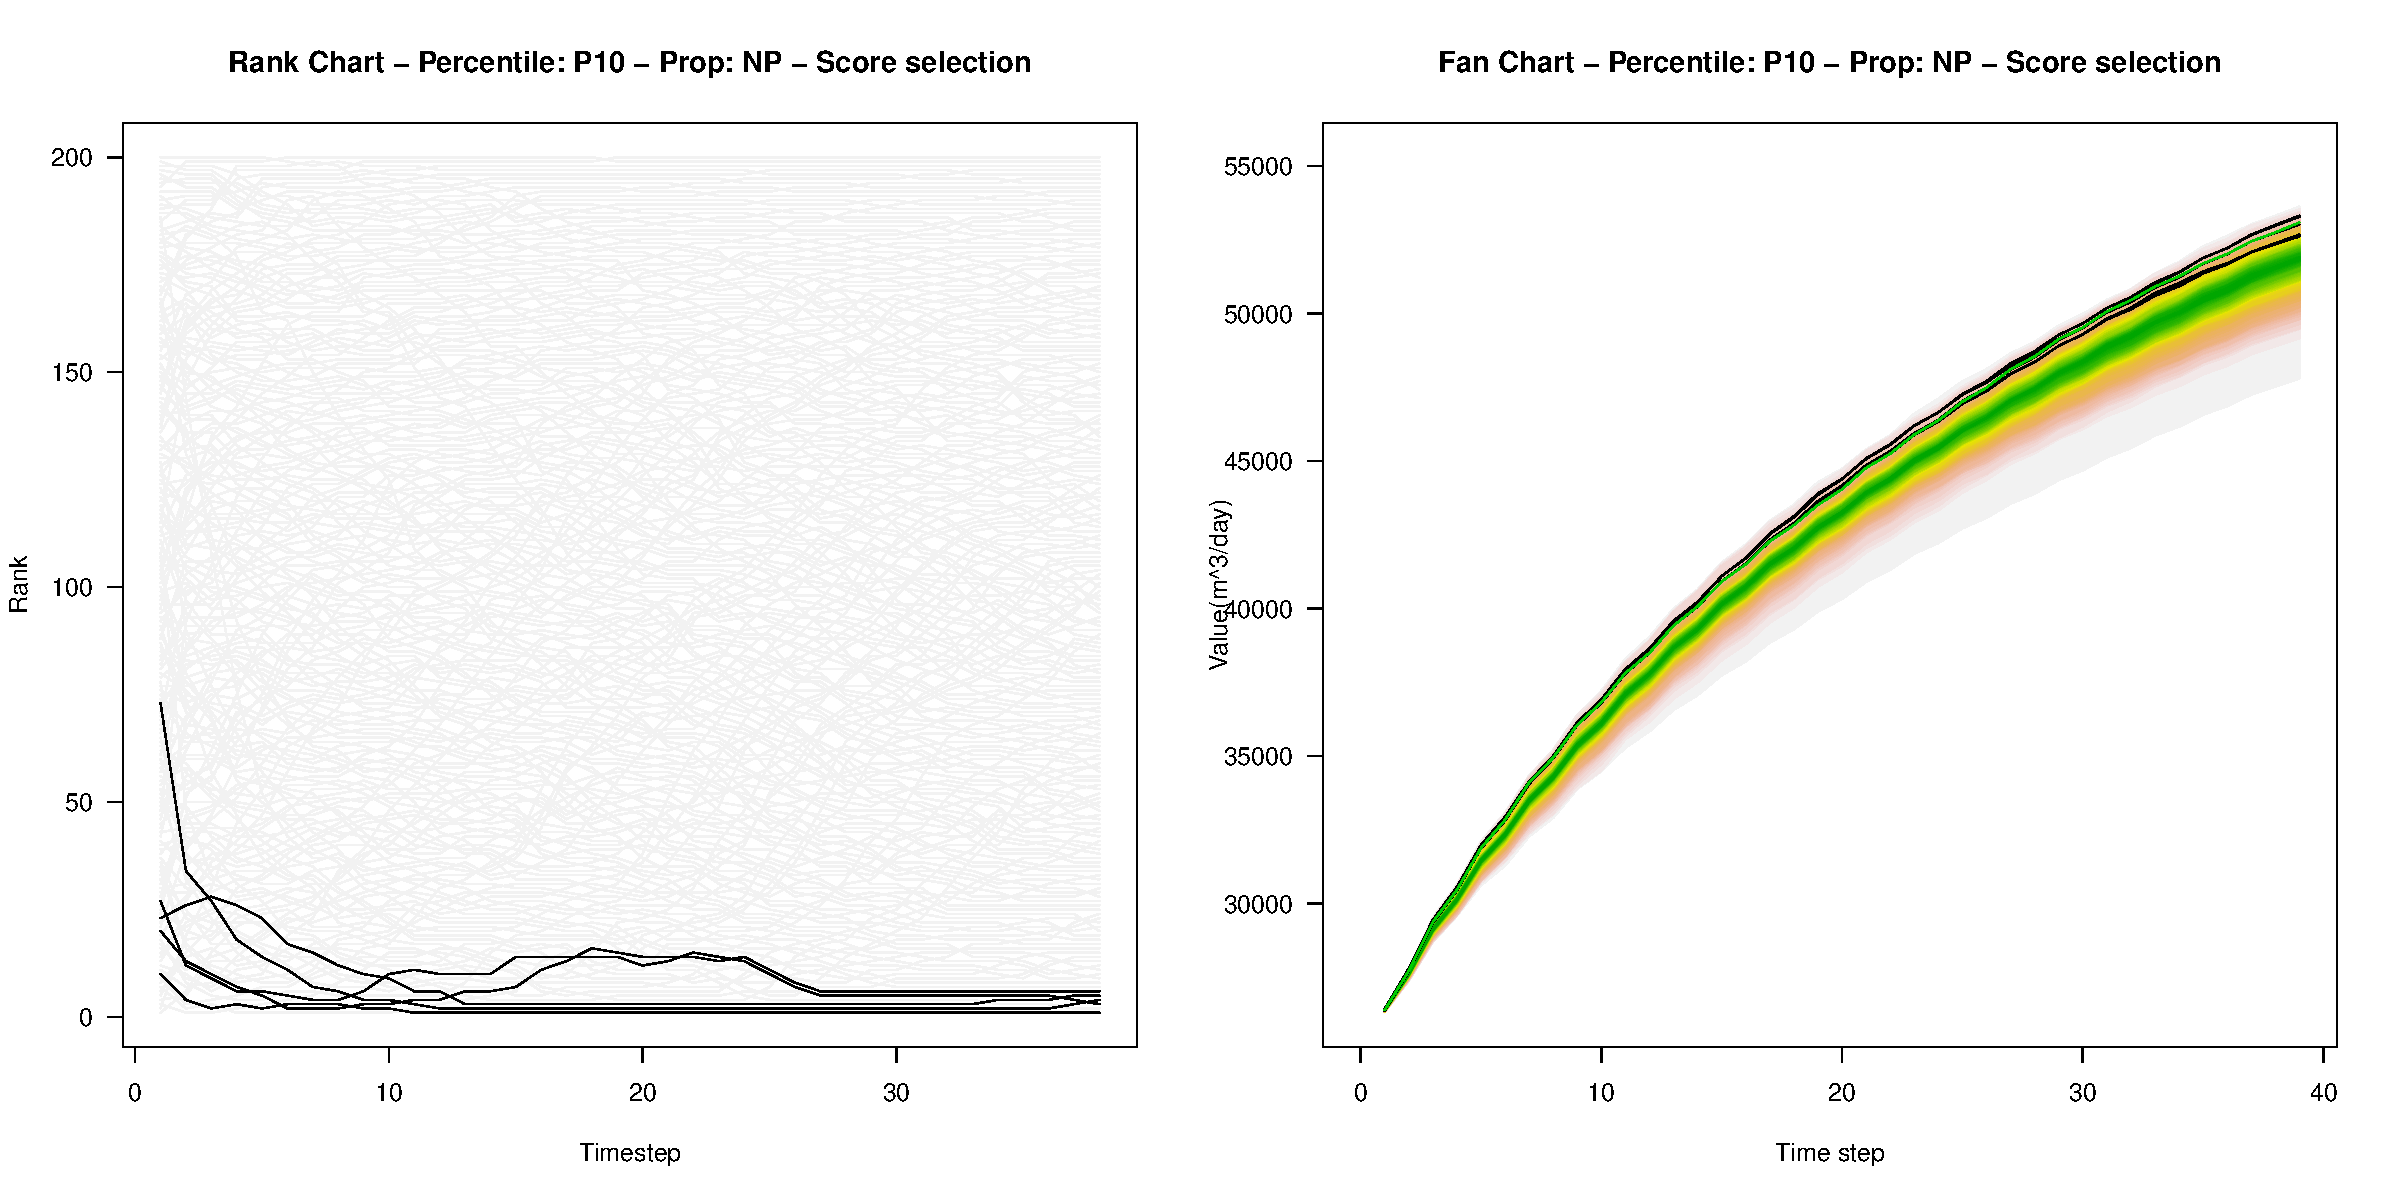
\includegraphics[width=0.9\columnwidth]{rank-fan-score-p10.pdf}
    \caption{Side-by-side rank and fan charts with the score selected curves highlighted. The selected models are UNISIM\_66, UNISIM\_156, UNISIM\_167, UNISIM\_87 and UNISIM\_54.}
    \label{fig:rank-fan-score-p10}
  \end{figure}
\end{frame}

\begin{frame}{Score-based Selection (P$_{50}$)}
  \begin{figure}[H]
    \centering
    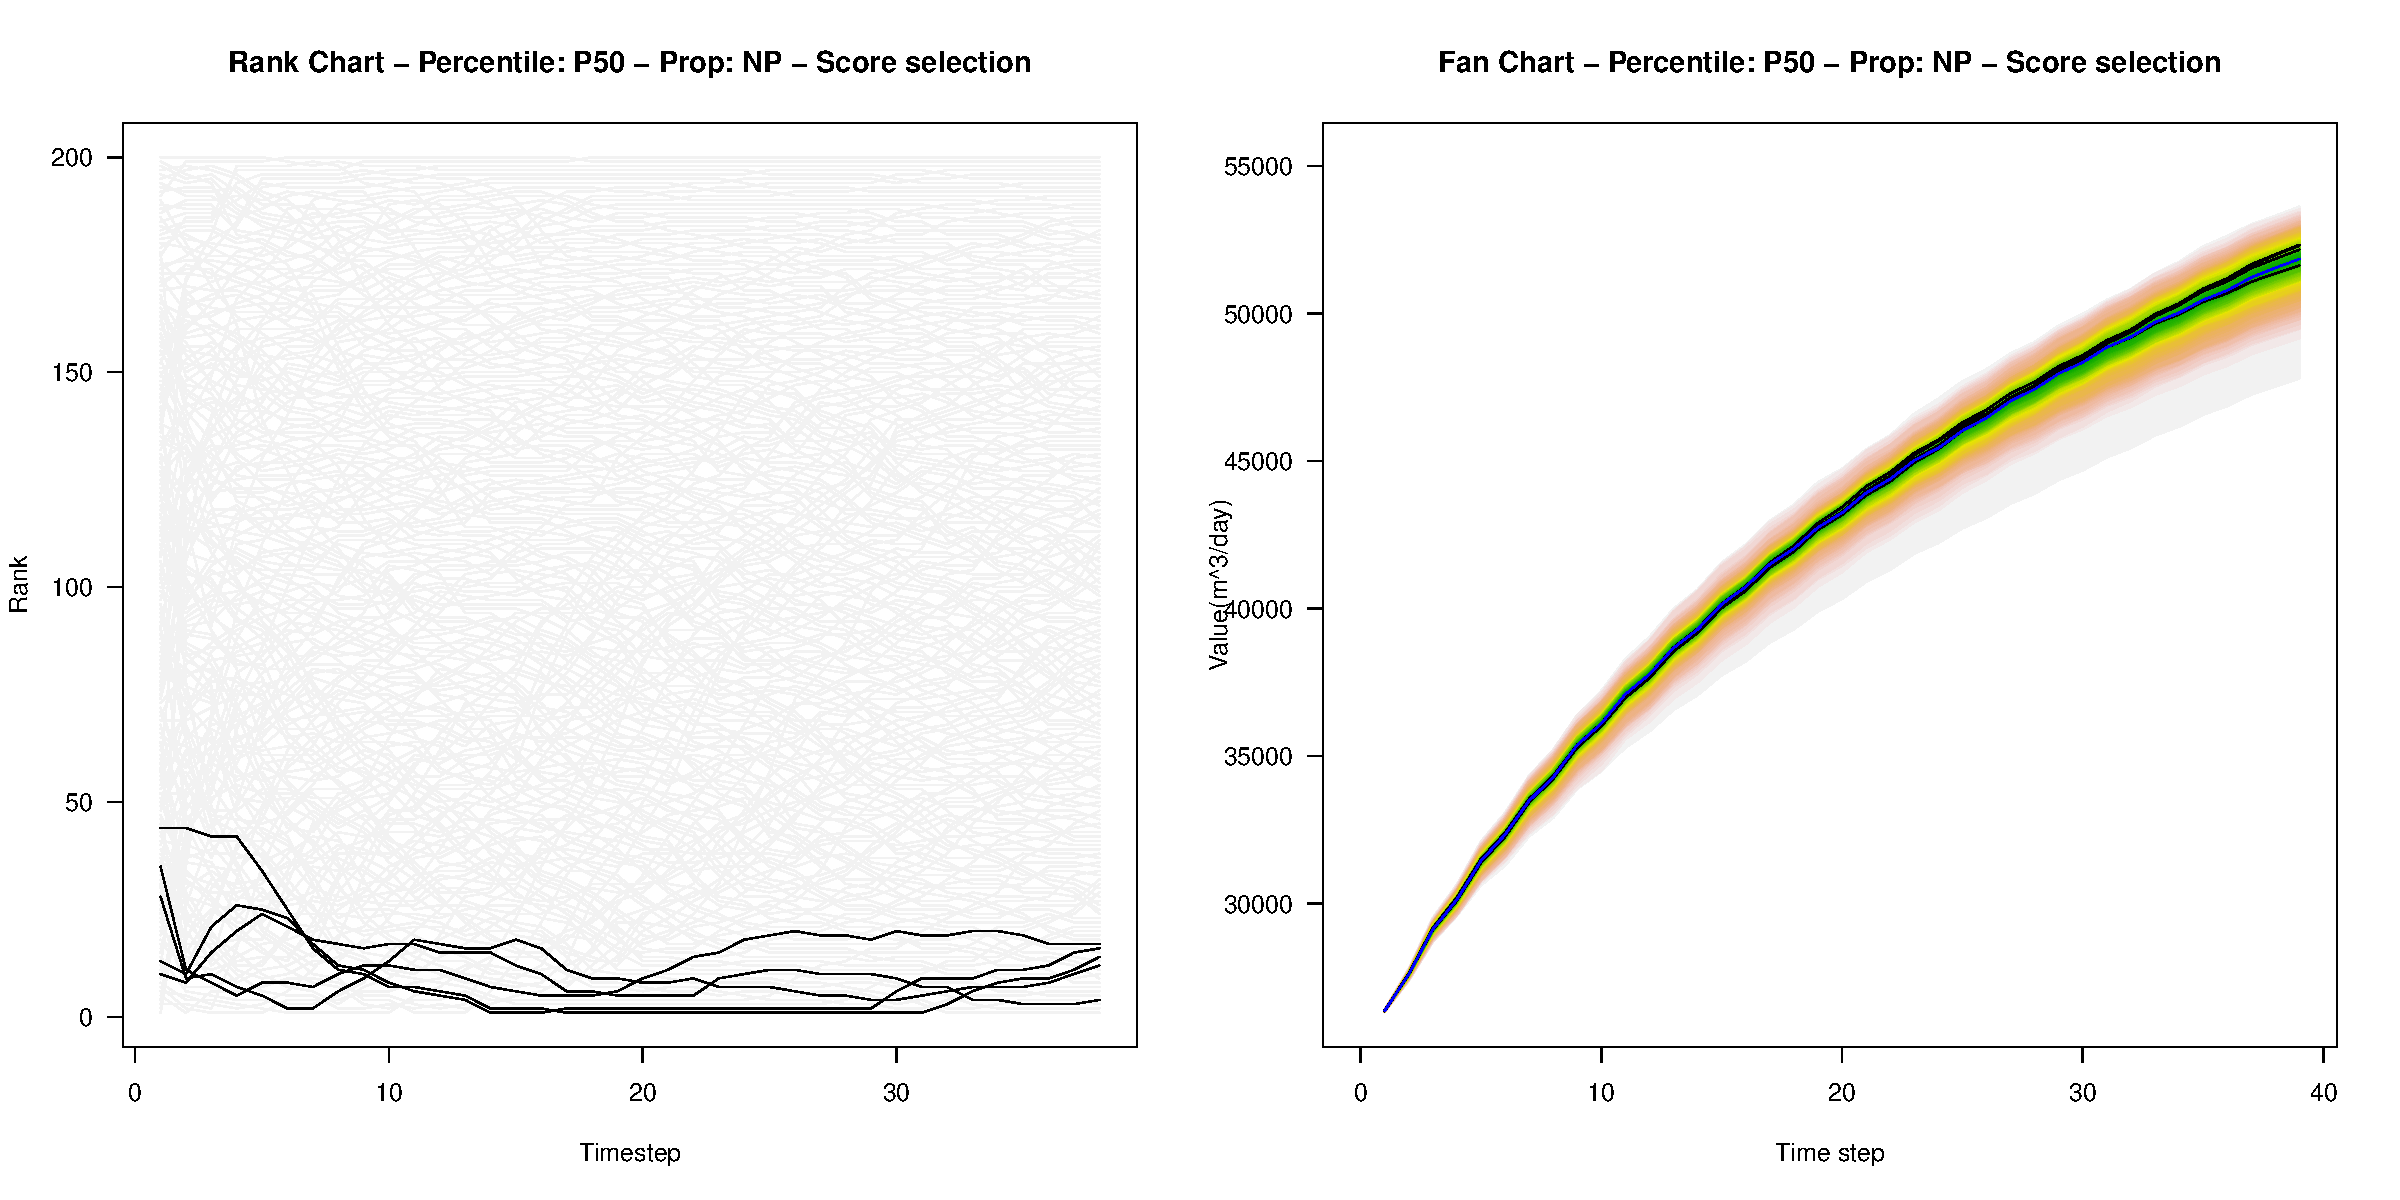
\includegraphics[width=0.9\columnwidth]{rank-fan-score-p50.pdf}
    \caption{Side-by-side rank and fan charts with the score selected curves highlighted. The selected models are UNISIM\_71, UNISIM\_30, UNISIM\_174, UNISIM\_45 and UNISIM\_135.}
    \label{fig:rank-fan-score-p50}
  \end{figure}
\end{frame}

\begin{frame}{Score-based Selection (P$_{90}$)}
  \begin{figure}[H]
    \centering
    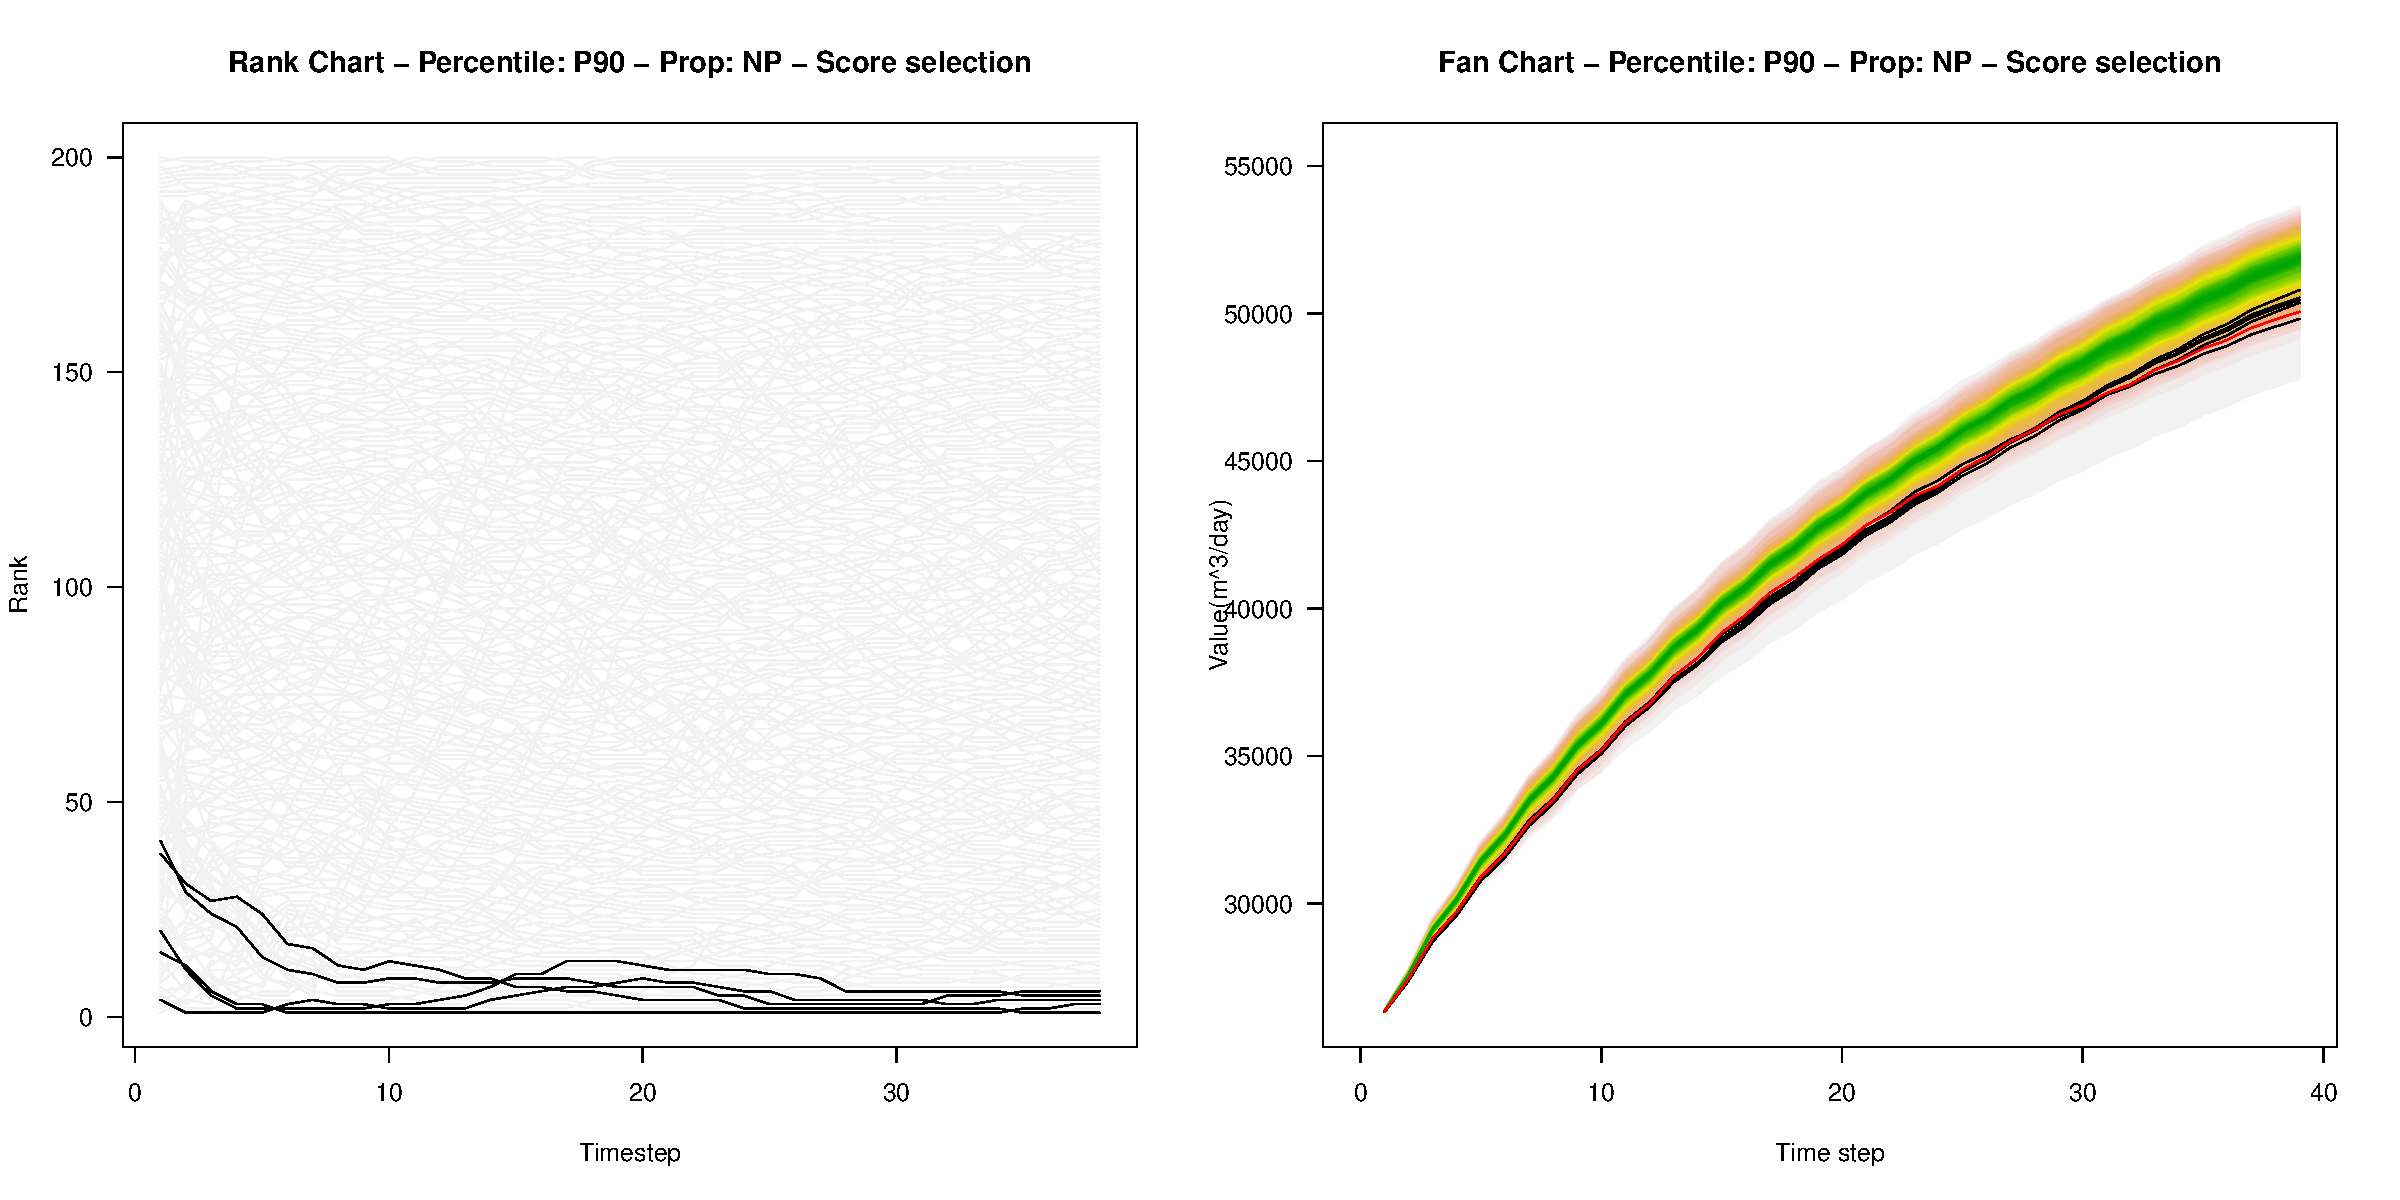
\includegraphics[width=0.9\columnwidth]{rank-fan-score-p90.pdf}
    \caption{Side-by-side rank and fan charts with the score selected curves highlighted. The selected models are UNISIM\_147, UNISIM\_58, UNISIM\_53, UNISIM\_186 and UNISIM\_111.}
    \label{fig:rank-fan-score-p90}
  \end{figure}
\end{frame}

\subsection{Brushing and Linking Selection}
\begin{frame}{Brushing and Linking Selecion}
  \begin{itemize}
    \item Technique developed to link multiple views of the same data;
    \item The idea is to brush a scenario in one view, and that scenario will be highlighted in the other views;
    \item The goal is to help the analysis by linking several views in order to provide a composed view of the data.
  \end{itemize}
\end{frame}

\begin{frame}{Brushing and Linking Selecion (Scenario/Distance Charts)}
  \begin{figure}[H]
    \centering
    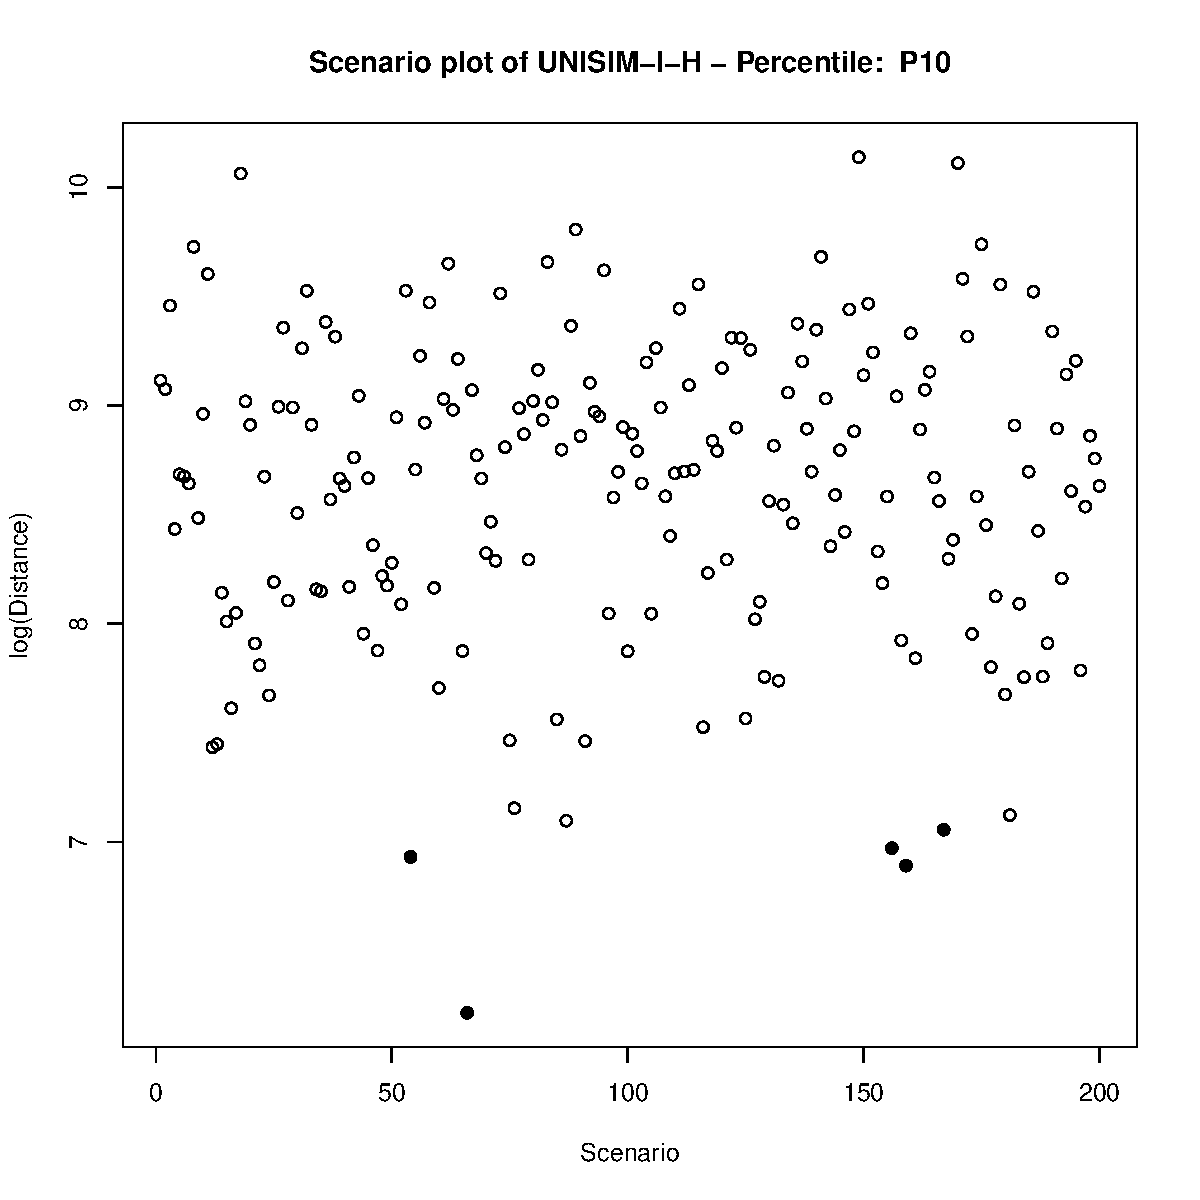
\includegraphics[width=0.33\columnwidth]{scen-NP-p10-log.pdf}
    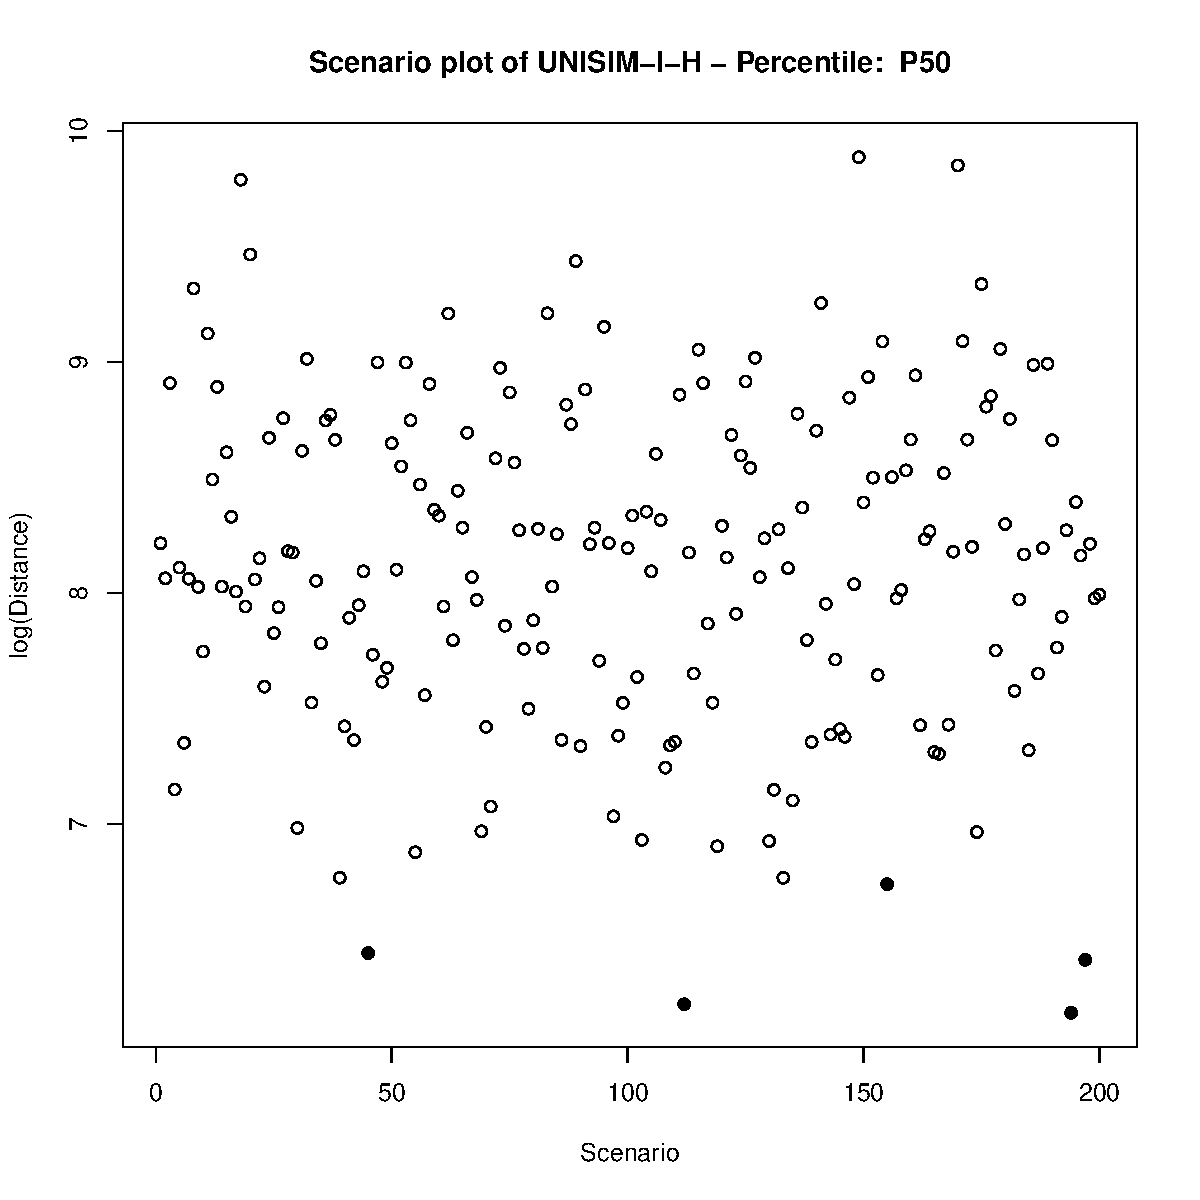
\includegraphics[width=0.33\columnwidth]{scen-NP-p50-log.pdf}
    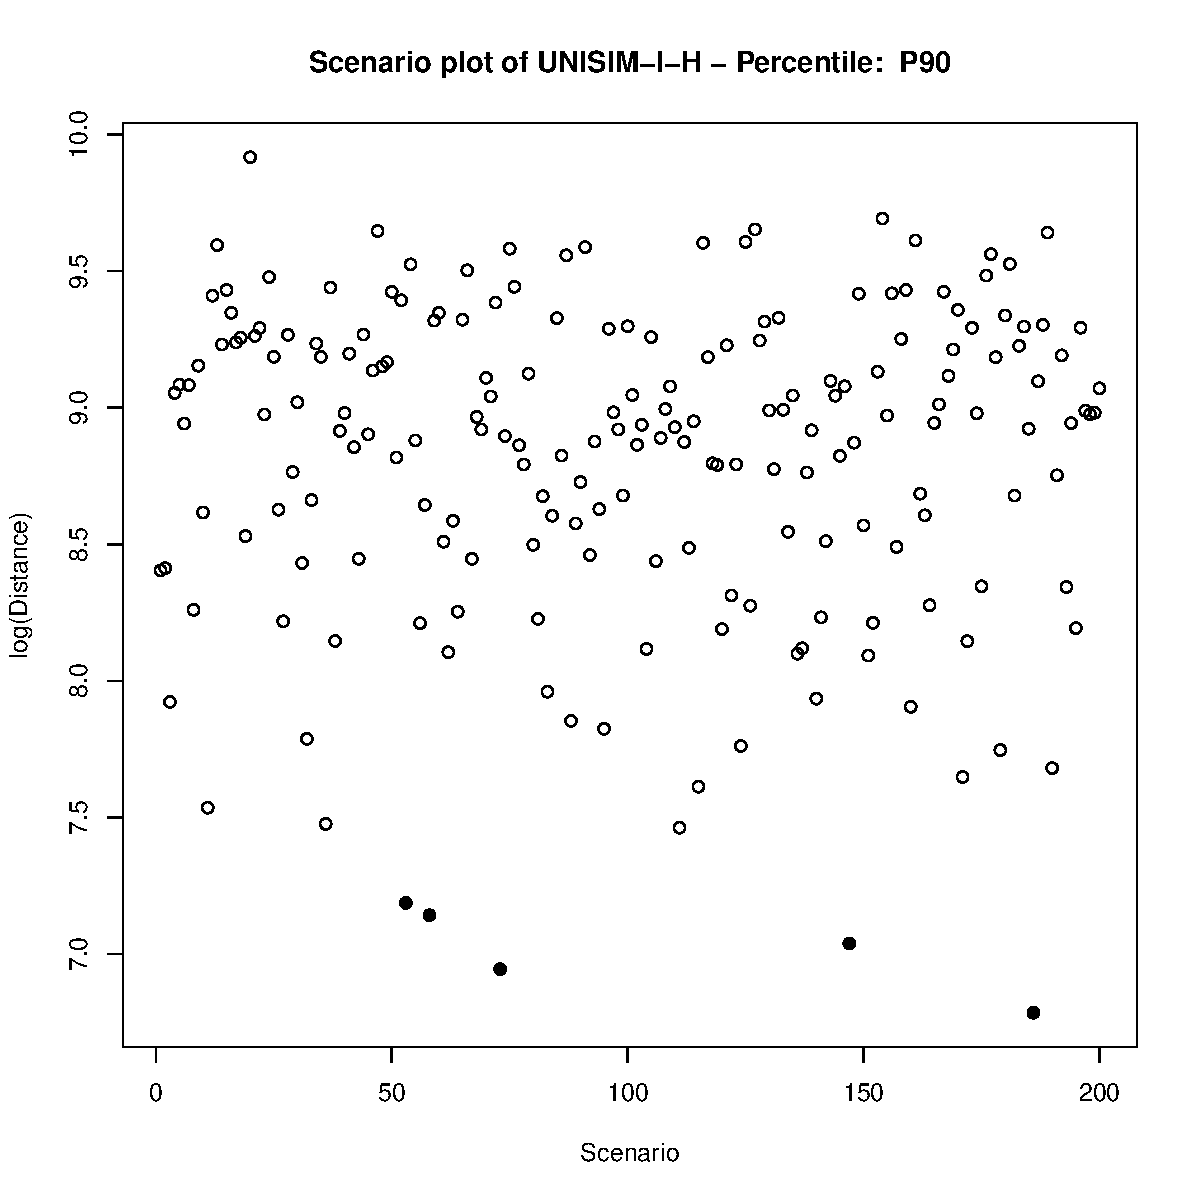
\includegraphics[width=0.33\columnwidth]{scen-NP-p90-log.pdf}
    \caption{Scenario charts of the manually selected curves. The $y$ axis is in logarithmic scale to ease the interpretation.}
    \label{fig:scen-brush}
  \end{figure}
\end{frame}

\begin{frame}{Brushing and Linking Selecion (P$_{10}$)}
  \begin{figure}[H]
    \centering
    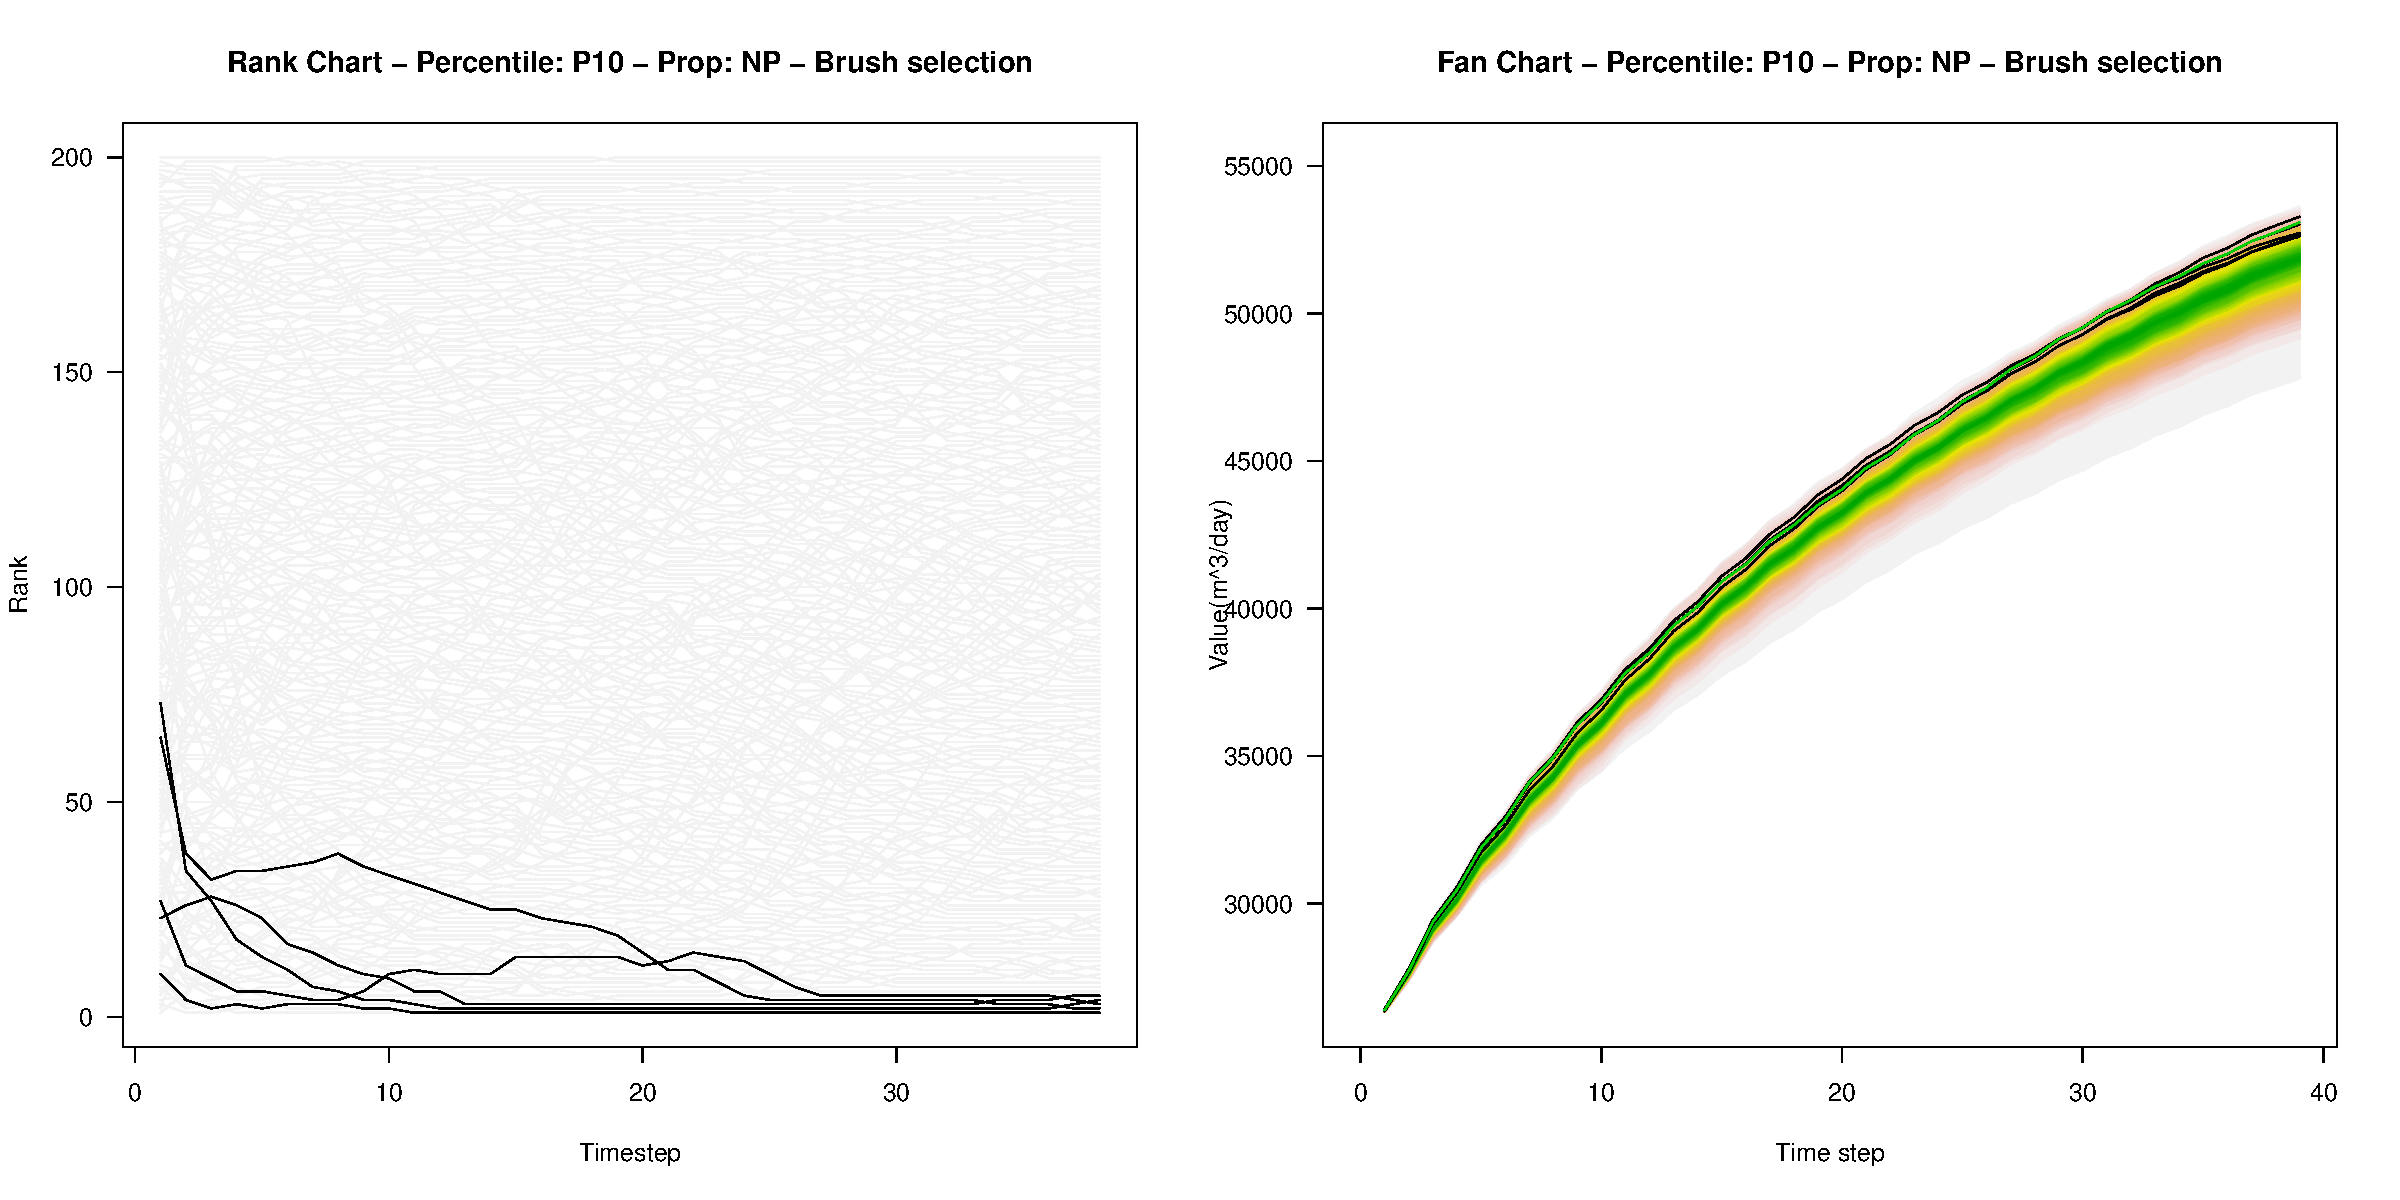
\includegraphics[width=0.9\columnwidth]{rank-fan-brush-p10.pdf}
    \caption{Side-by-side rank and fan charts with the manually selected curves highlighted. The selected models are UNISIM\_66, UNISIM\_159, UNISIM\_54, UNISIM\_156 and UNISIM\_167.}
    \label{fig:rank-fan-brush-p10}
  \end{figure}
\end{frame}

\begin{frame}{Brushing and Linking Selecion (P$_{50}$)}
  \begin{figure}[H]
    \centering
    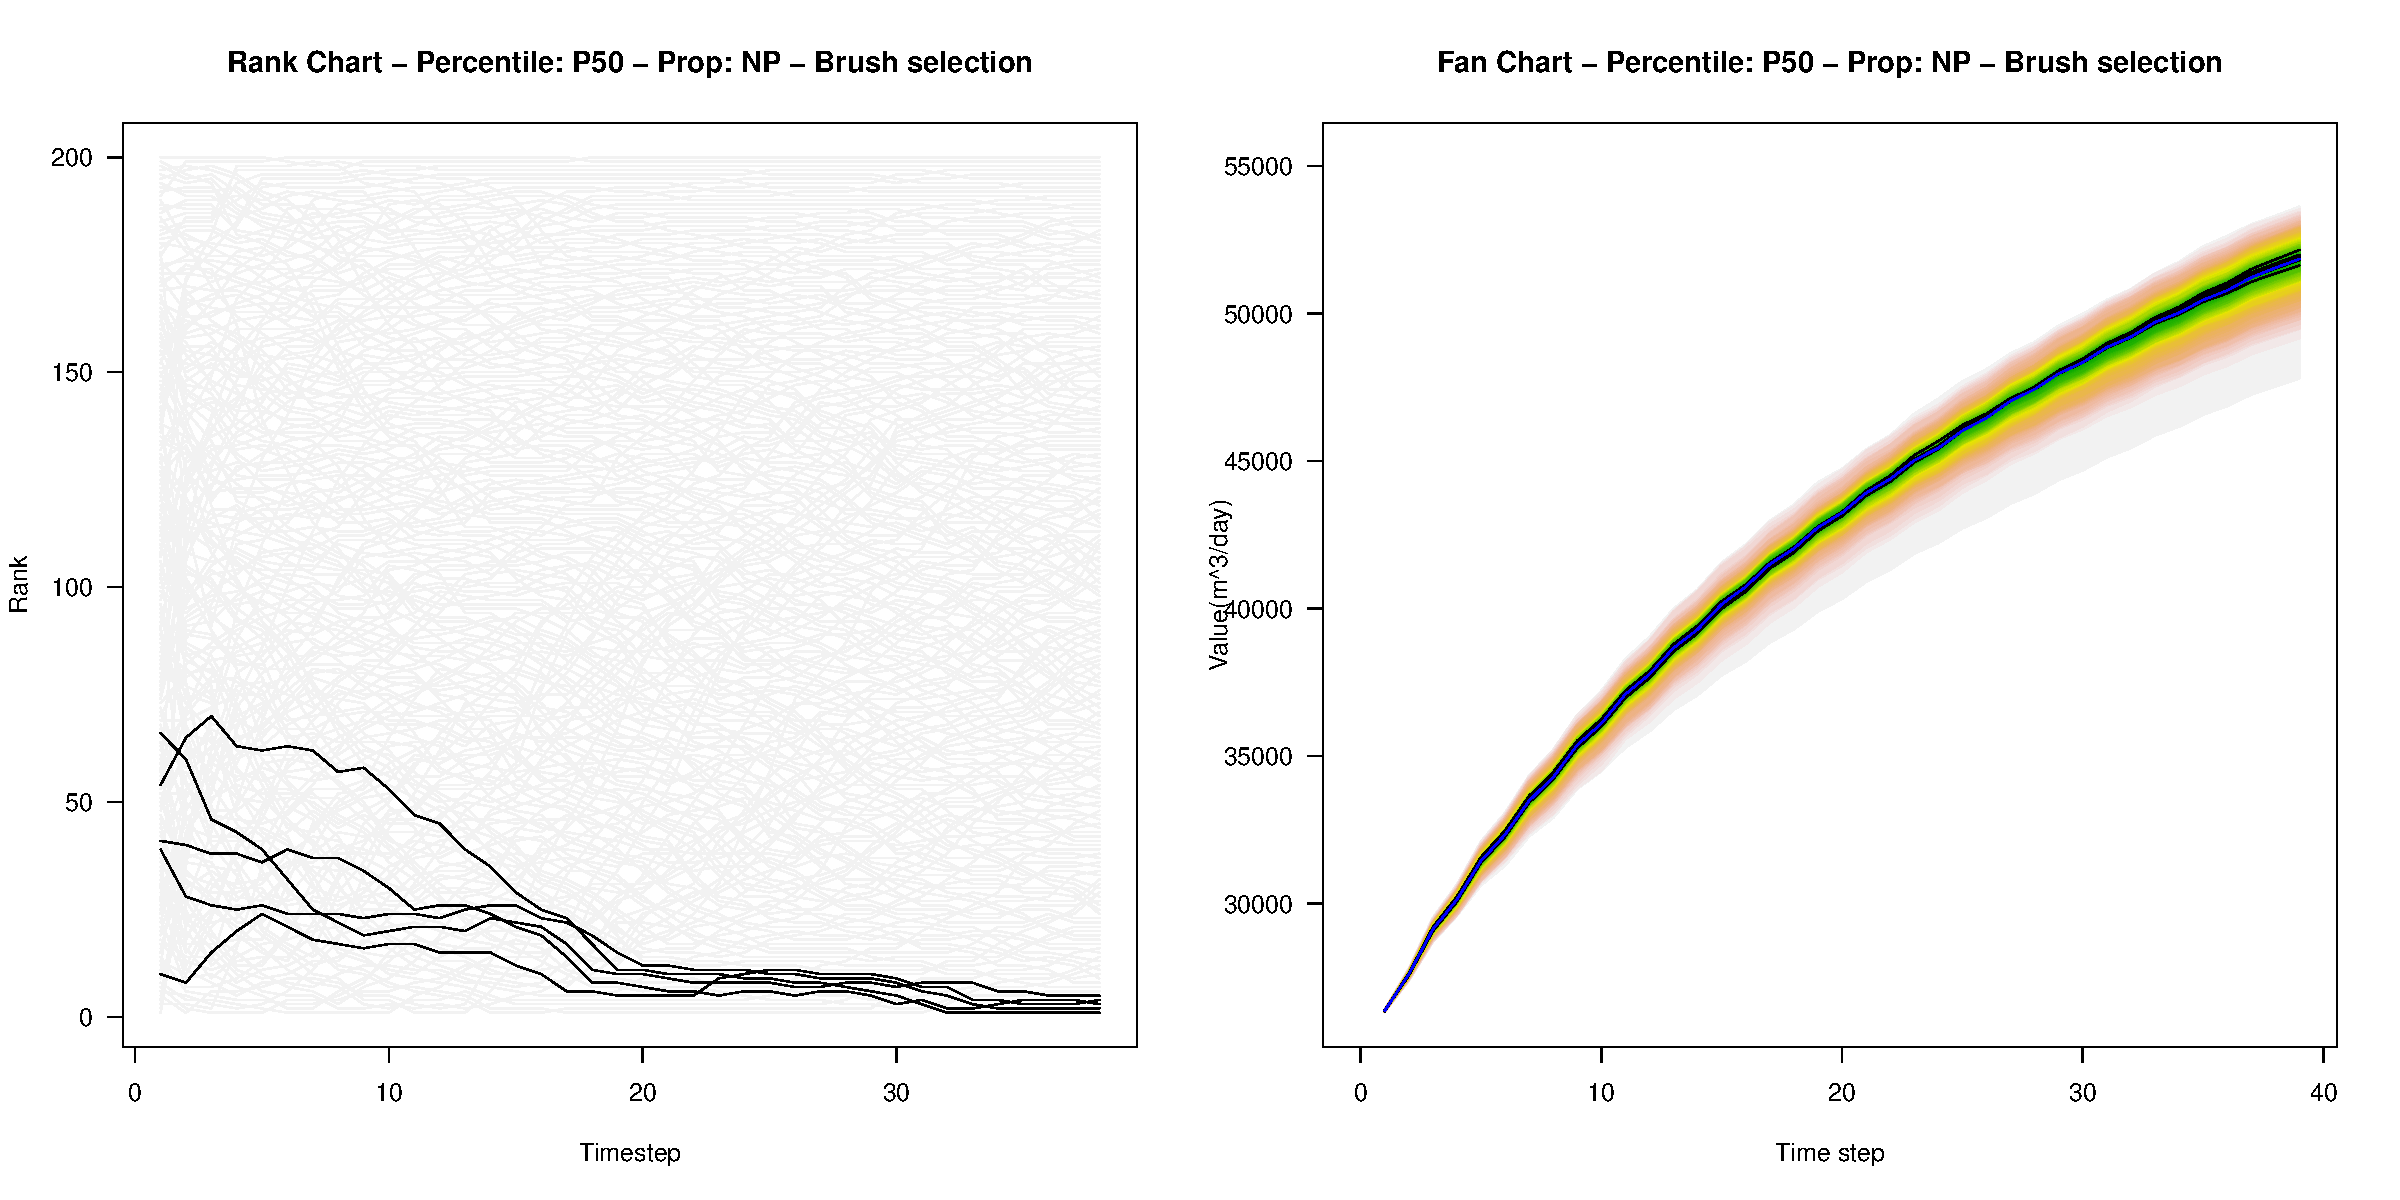
\includegraphics[width=0.9\columnwidth]{rank-fan-brush-p50.pdf}
    \caption{Side-by-side rank and fan charts with the manually selected curves highlighted. The selected models are UNISIM\_194, UNISIM\_112, UNISIM\_197, UNISIM\_45 and UNISIM\_155.}
    \label{fig:rank-fan-brush-p50}
  \end{figure}
\end{frame}

\begin{frame}{Brushing and Linking Selecion (P$_{90}$)}
  \begin{figure}[H]
    \centering
    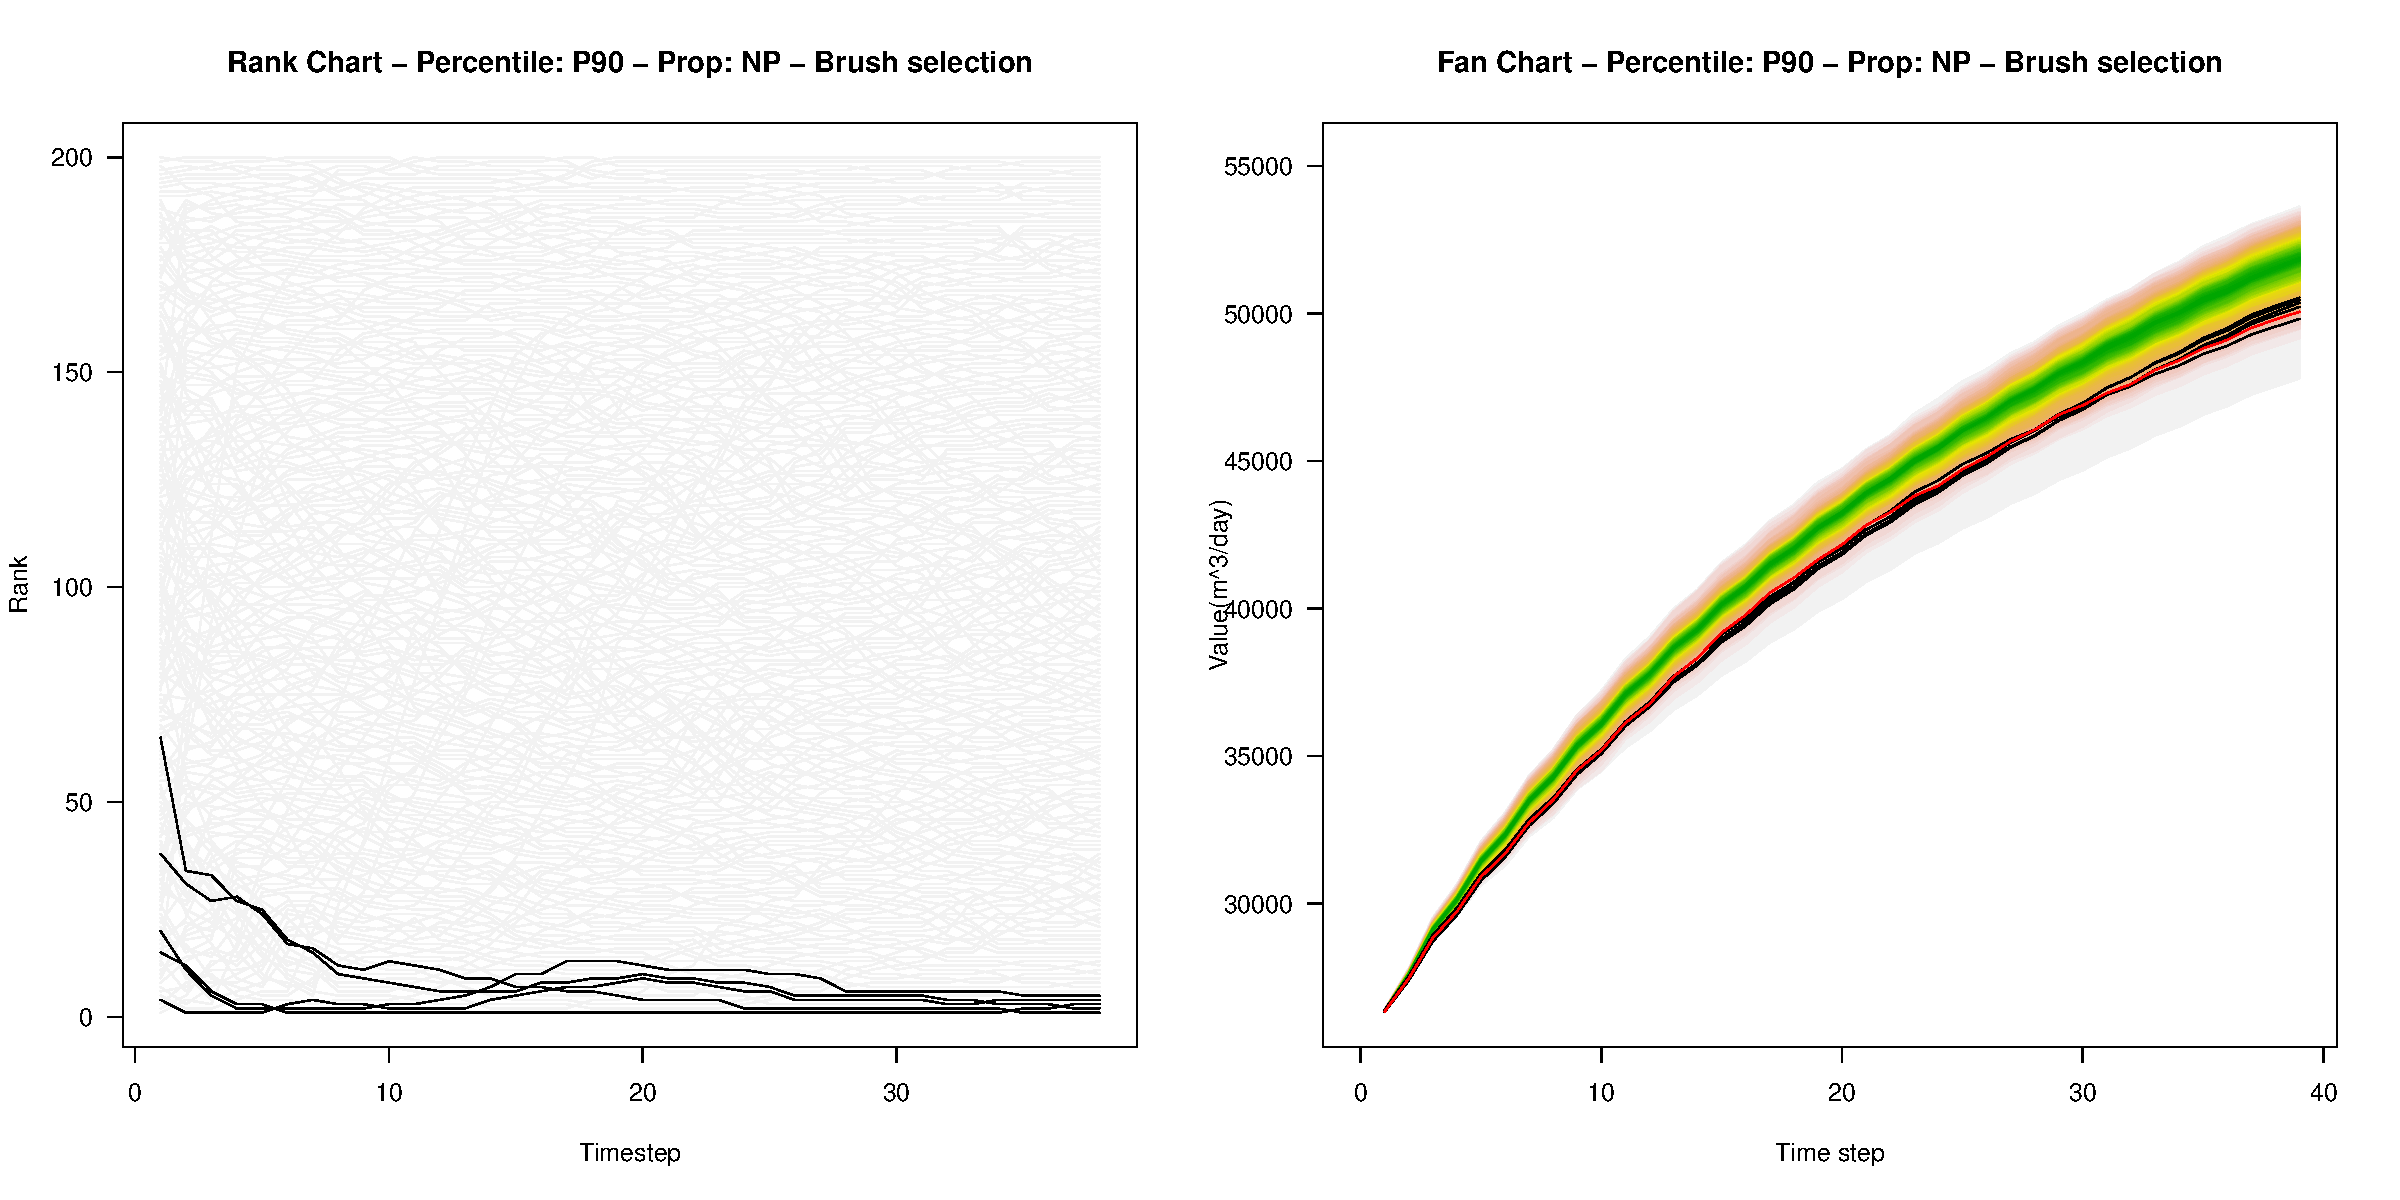
\includegraphics[width=0.9\columnwidth]{rank-fan-brush-p90.pdf}
    \caption{Side-by-side rank and fan charts with the manually selected curves highlighted. The selected models are UNISIM\_155 for P$_{50}$; and UNISIM\_186, UNISIM\_73, UNISIM\_147, UNISIM\_58 and UNISIM\_53.}
    \label{fig:rank-fan-brush-p90}
  \end{figure}
\end{frame}

\begin{frame}{Comparative MDS projections (P$_{10}$)}
  \begin{figure}[H]
    \centering
    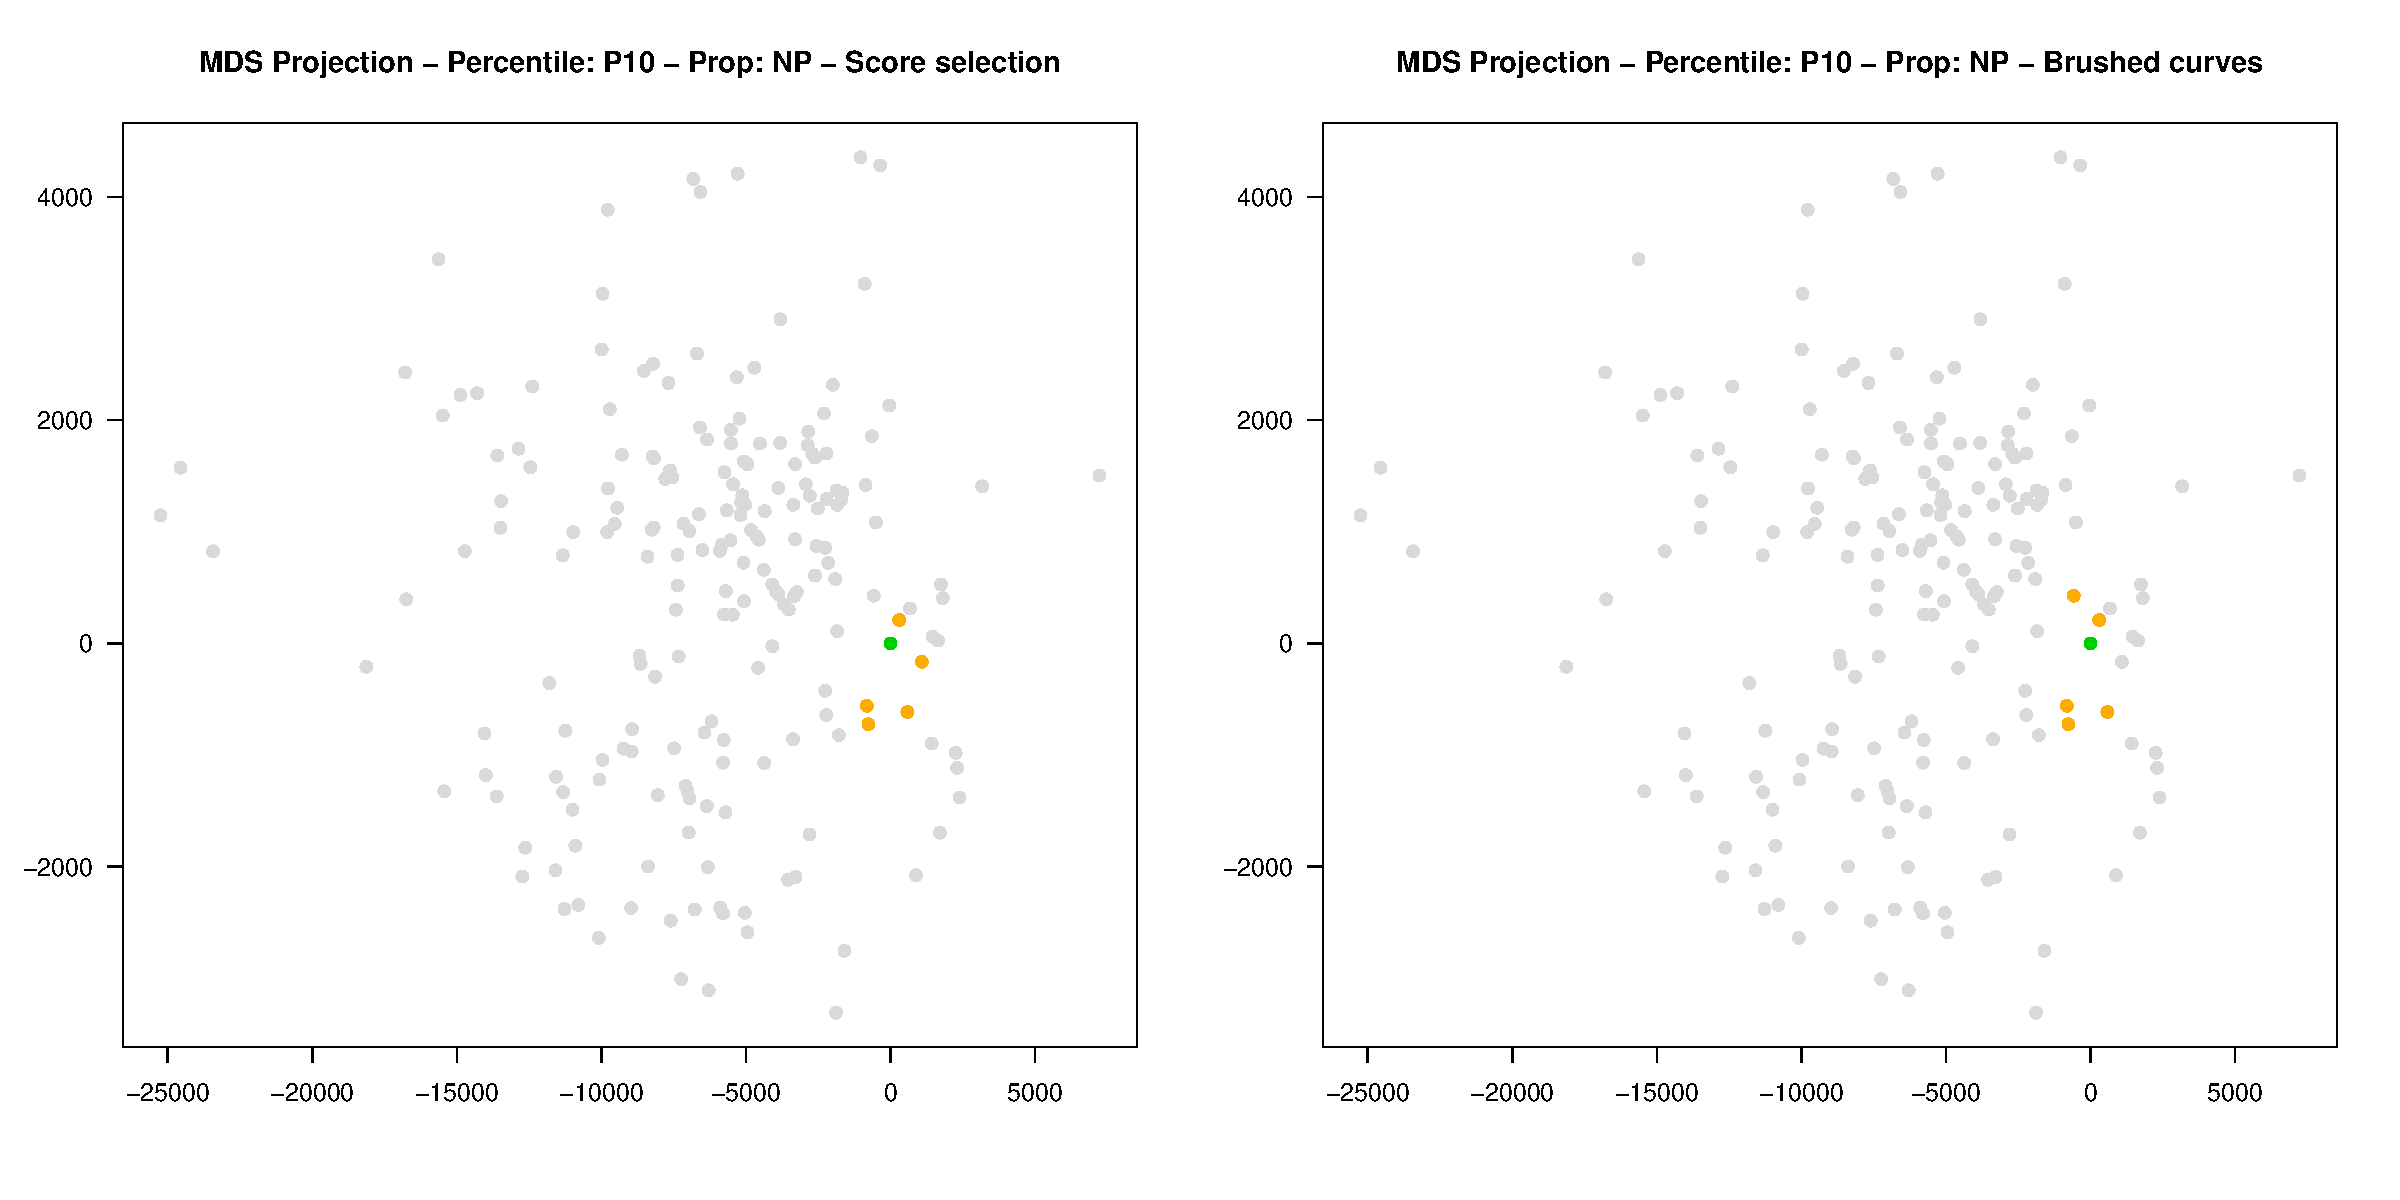
\includegraphics[width=0.9\columnwidth]{figures/mds-brush-score-p10.pdf}
    \caption{Comparative MDS projections of the sets selected by the score and manual brushing approaches.}
    \label{fig:mds-plots}
  \end{figure}
\end{frame}

\begin{frame}{Comparative MDS projections (P$_{50}$)}
  \begin{figure}[H]
    \centering
    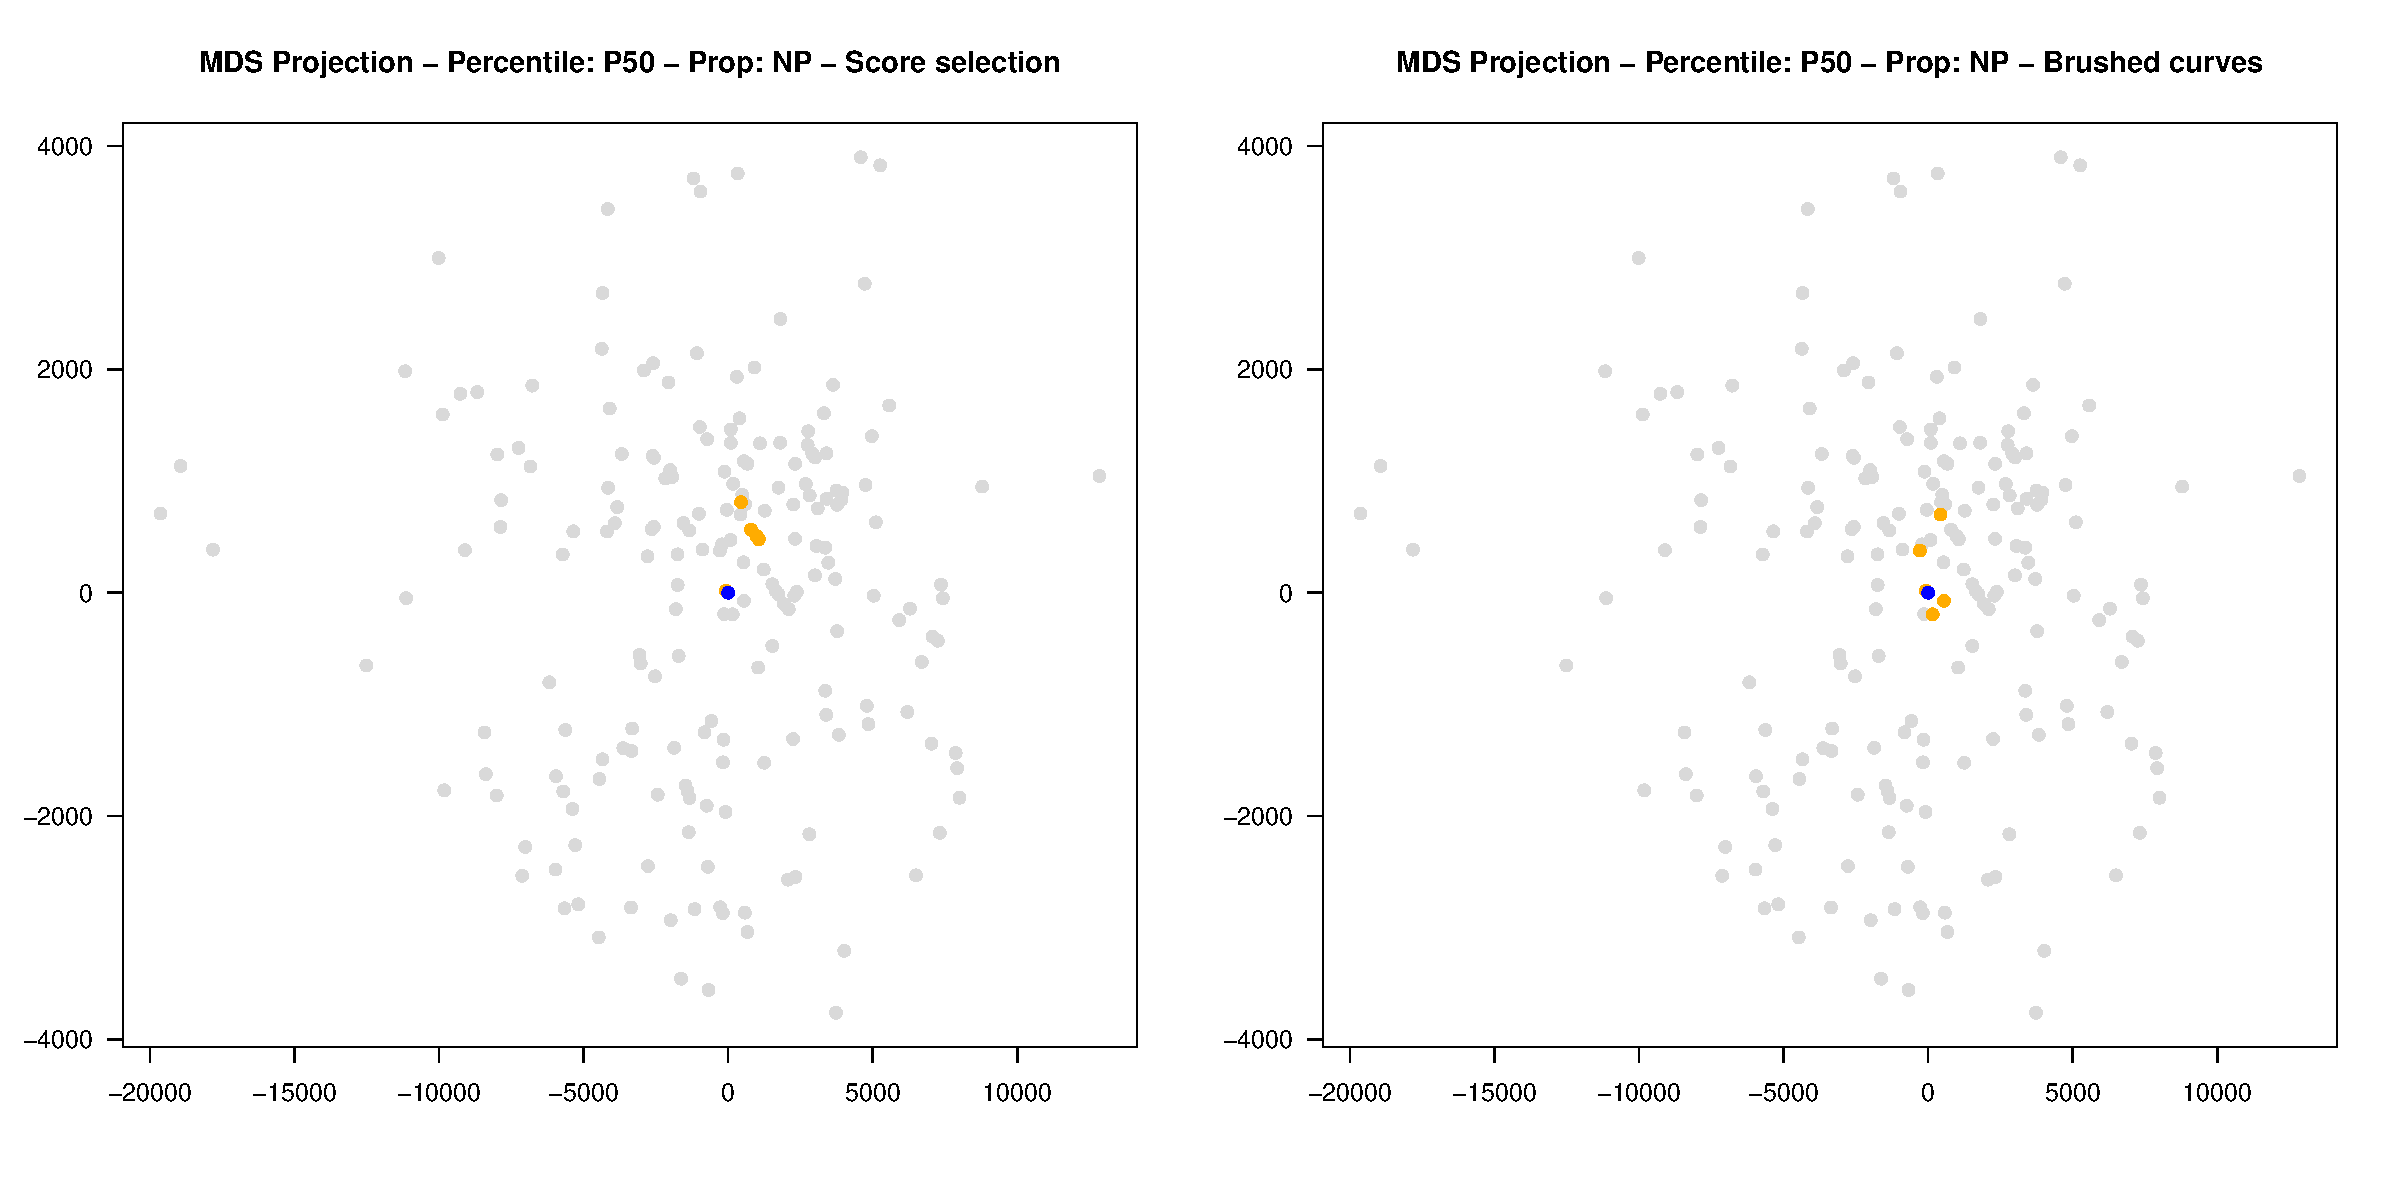
\includegraphics[width=0.9\columnwidth]{figures/mds-brush-score-p50.pdf}
    \caption{Comparative MDS projections of the sets selected by the score and manual brushing approaches.}
    \label{fig:mds-plots}
  \end{figure}
\end{frame}

\begin{frame}{Comparative MDS projections (P$_{90}$)}
  \begin{figure}[H]
    \centering
    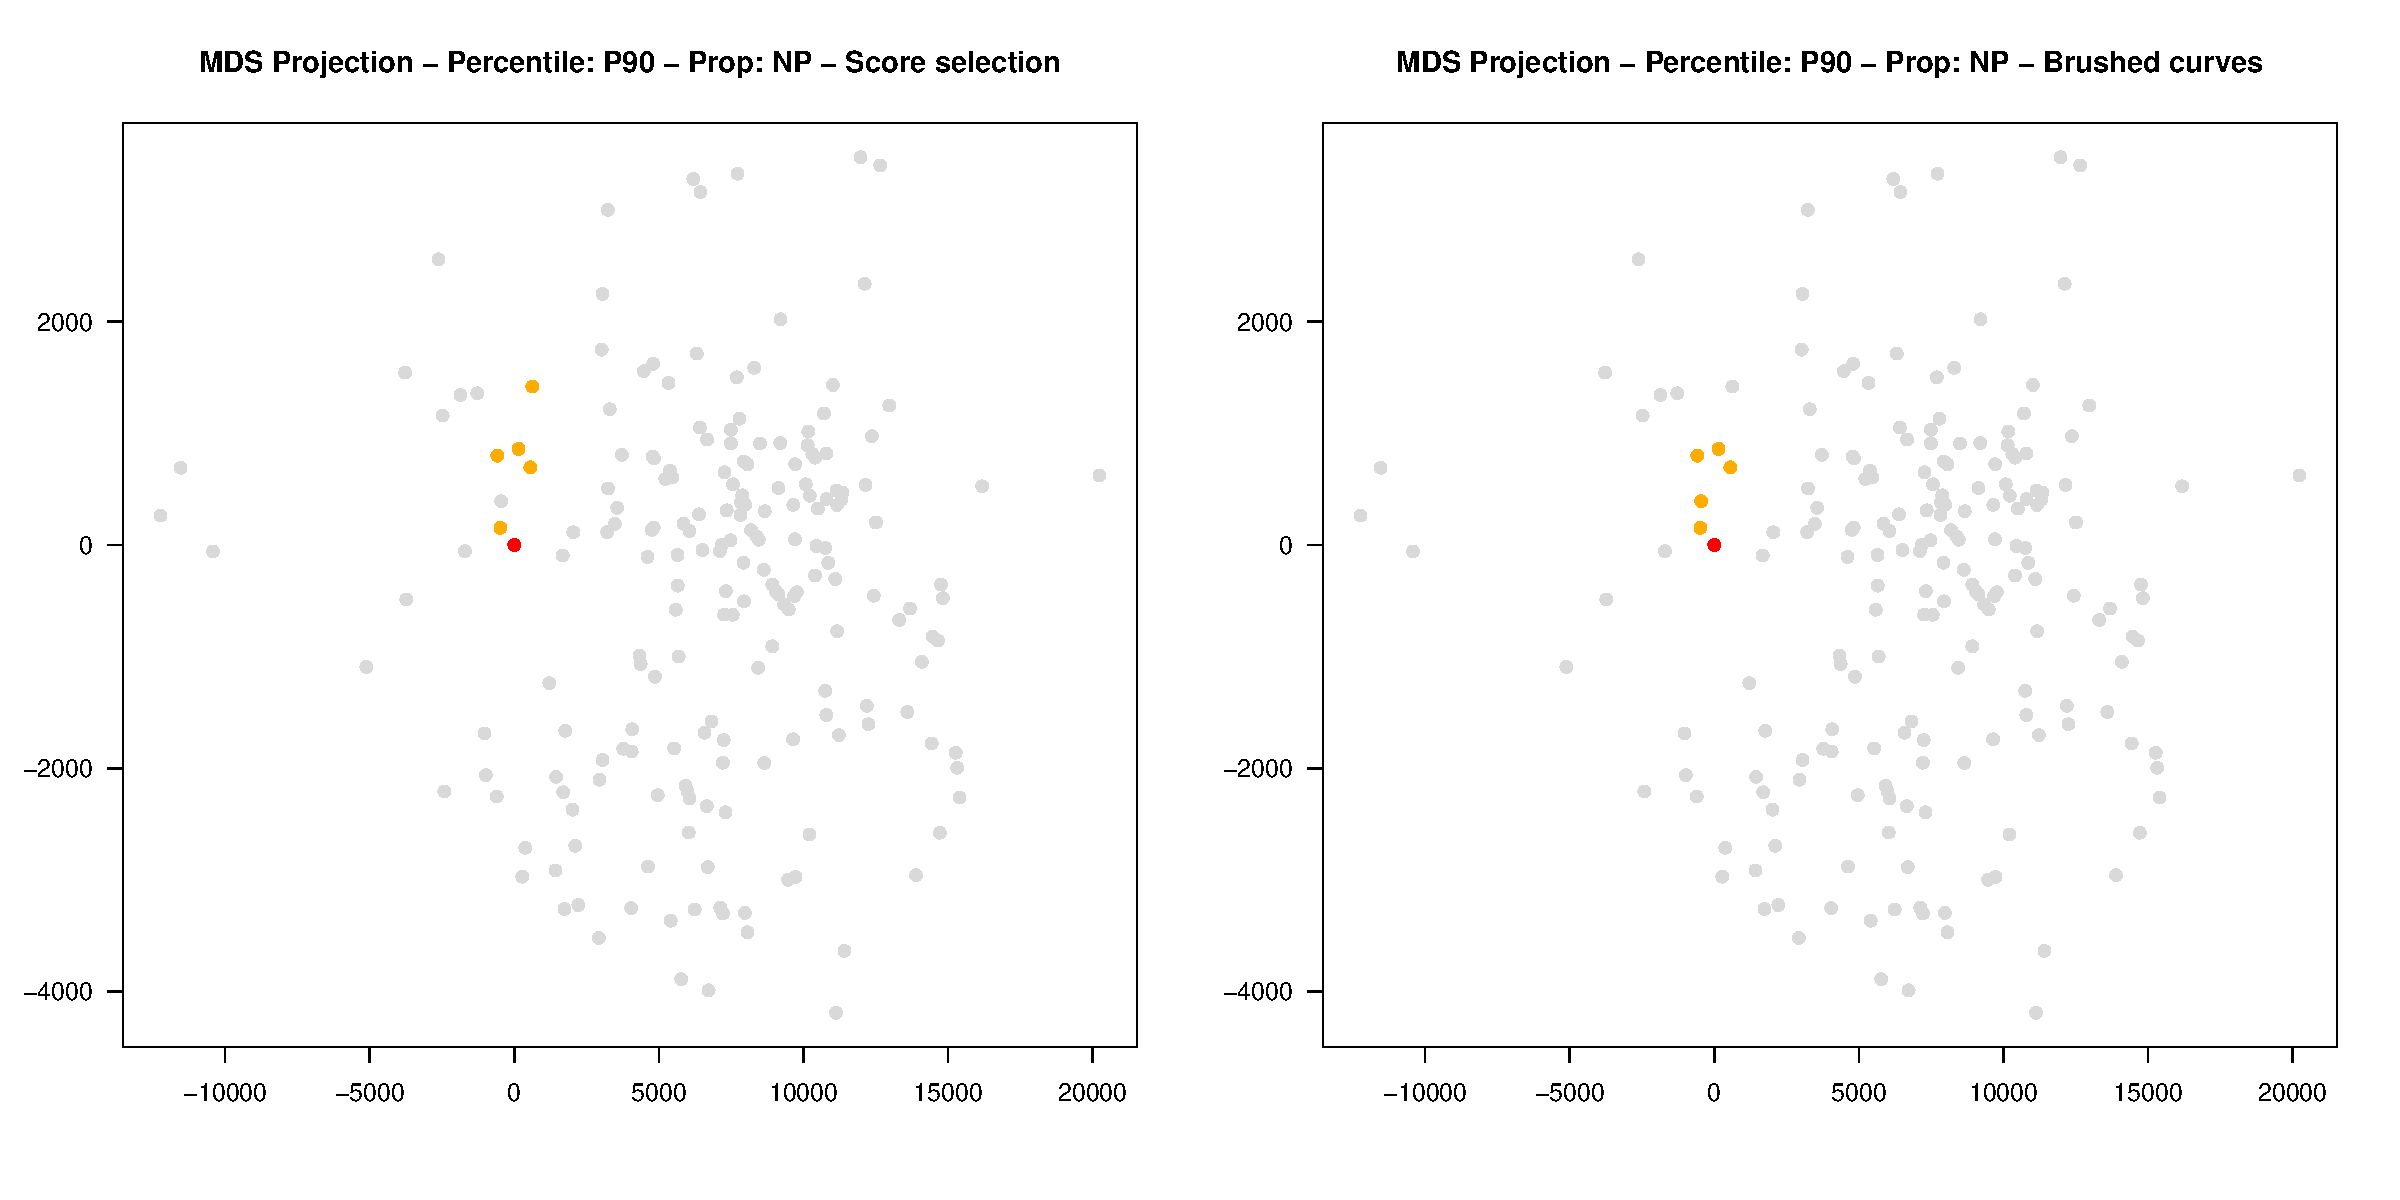
\includegraphics[width=0.9\columnwidth]{figures/mds-brush-score-p90.pdf}
    \caption{Comparative MDS projections of the sets selected by the score and manual brushing approaches.}
    \label{fig:mds-plots}
  \end{figure}
\end{frame}

\subsection{MDS kNN Selection}
\begin{frame}{MDS kNN Selection}
  \begin{itemize}
    \item By comparing the MDS projections of the models, both approaches leave some of the closest models out of the selection;
    \item We executed a kNN selection based on the projections of the models to investigate the behaviors of the modelos closest to the percentiles;
  \end{itemize}
\end{frame}

\begin{frame}{MDS kNN Selection (P$_{10}$)}
  \begin{figure}[H]
    \centering
    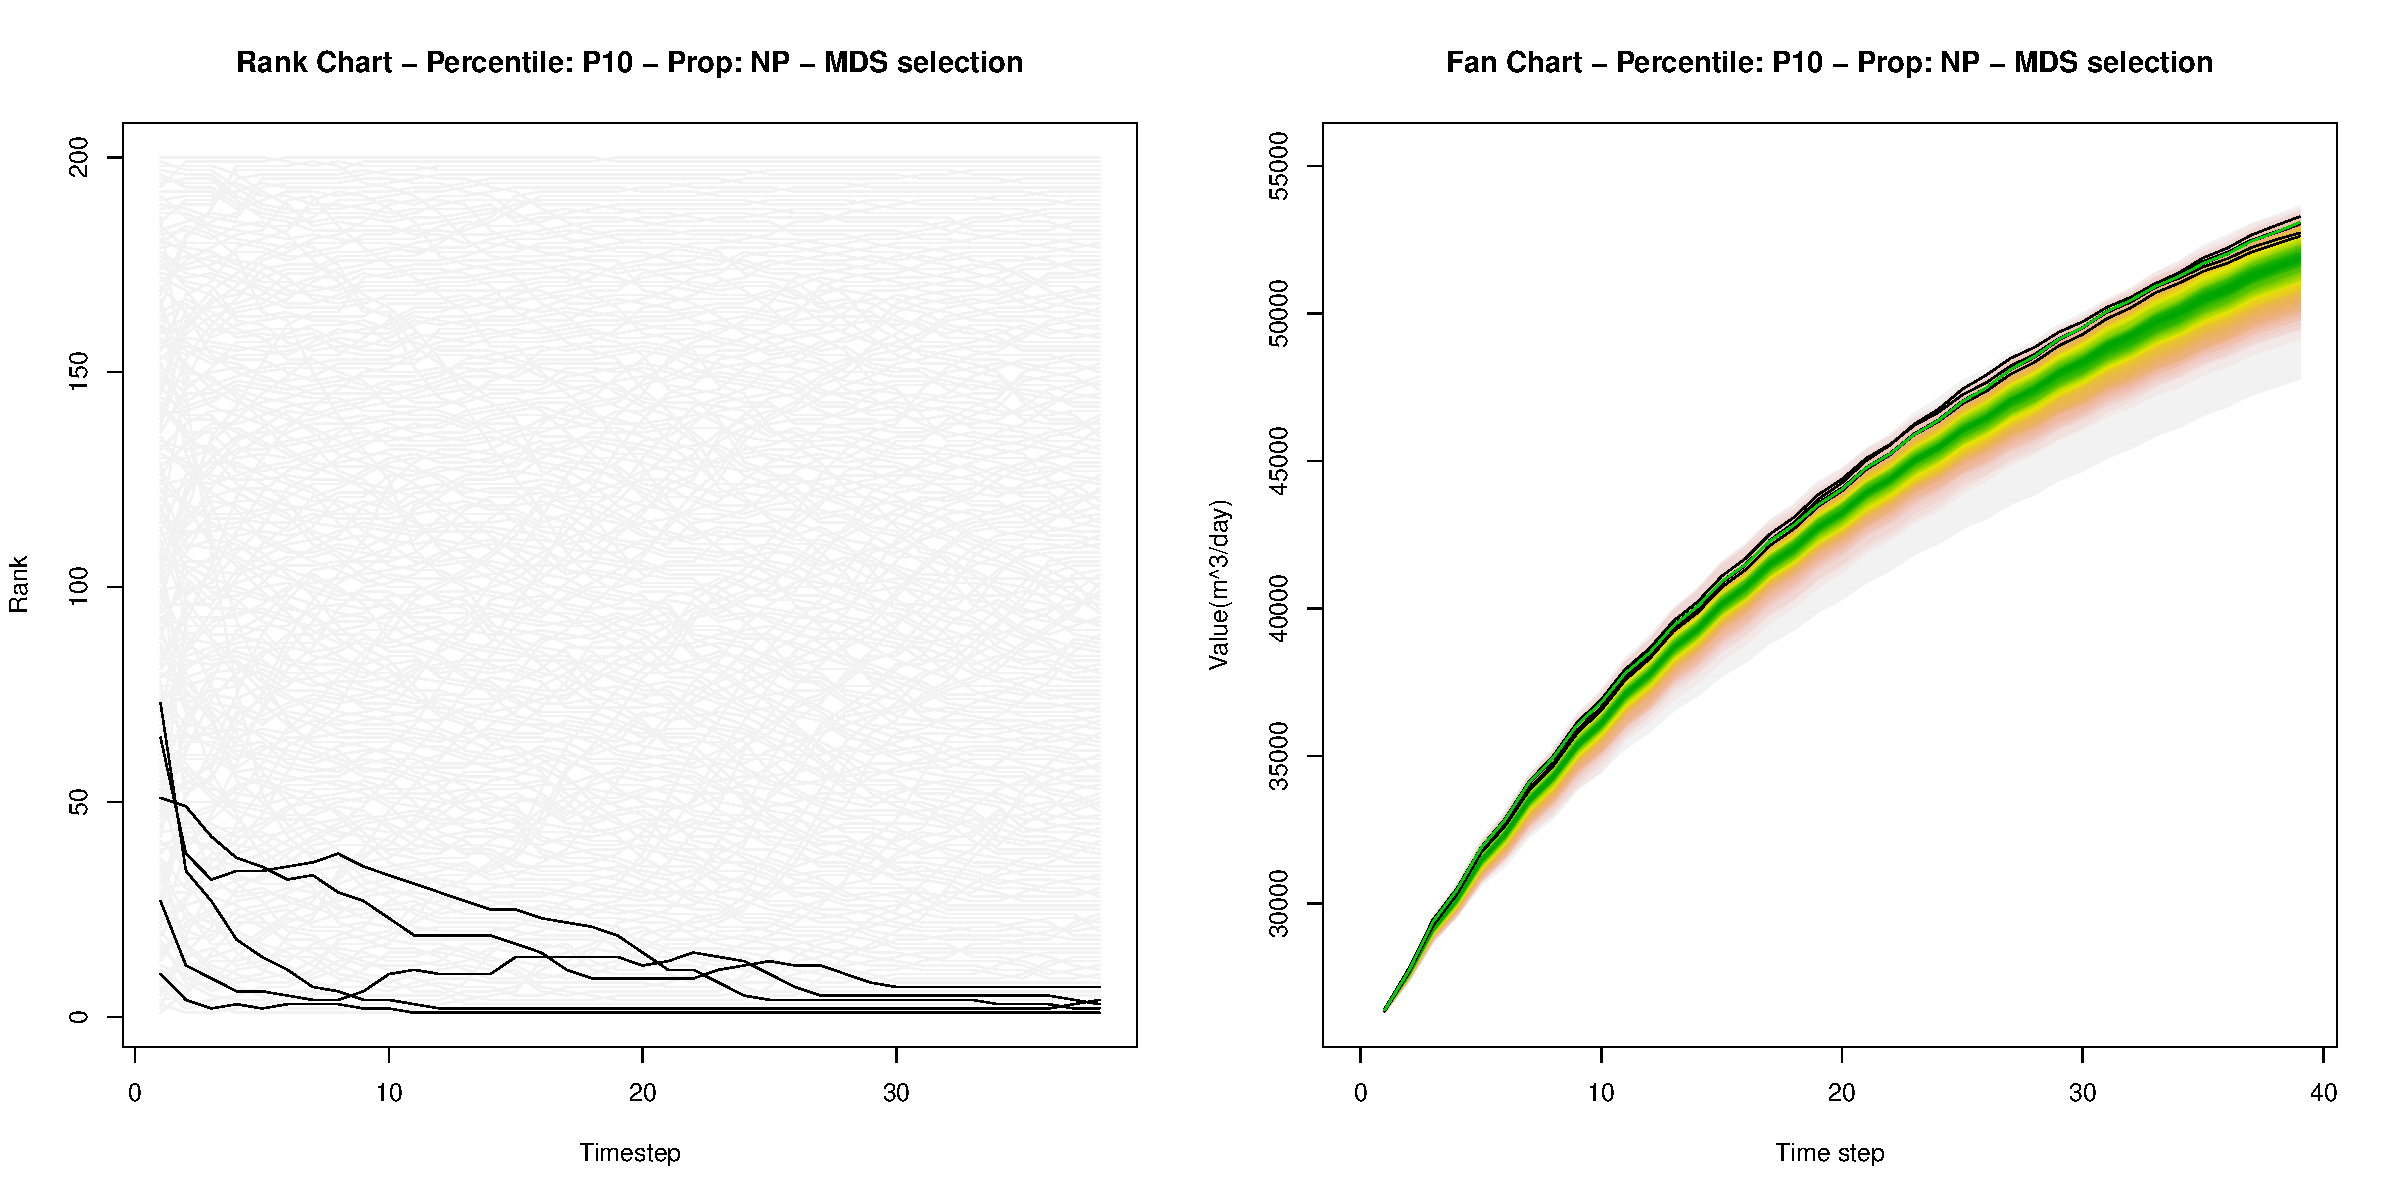
\includegraphics[width=0.9\columnwidth]{rank-fan-mds-sel-p10.pdf}
    \caption{Side-by-side rank and fan charts of the MDS projection selected curves. The selected models are UNISIM\_66, UNISIM\_159, UNISIM\_181, UNISIM\_54 and UNISIM\_156.}
    \label{fig:rank-fan-mds}
  \end{figure}
\end{frame}

\begin{frame}{MDS kNN Selection (P$_{50}$)}
  \begin{figure}[H]
    \centering
    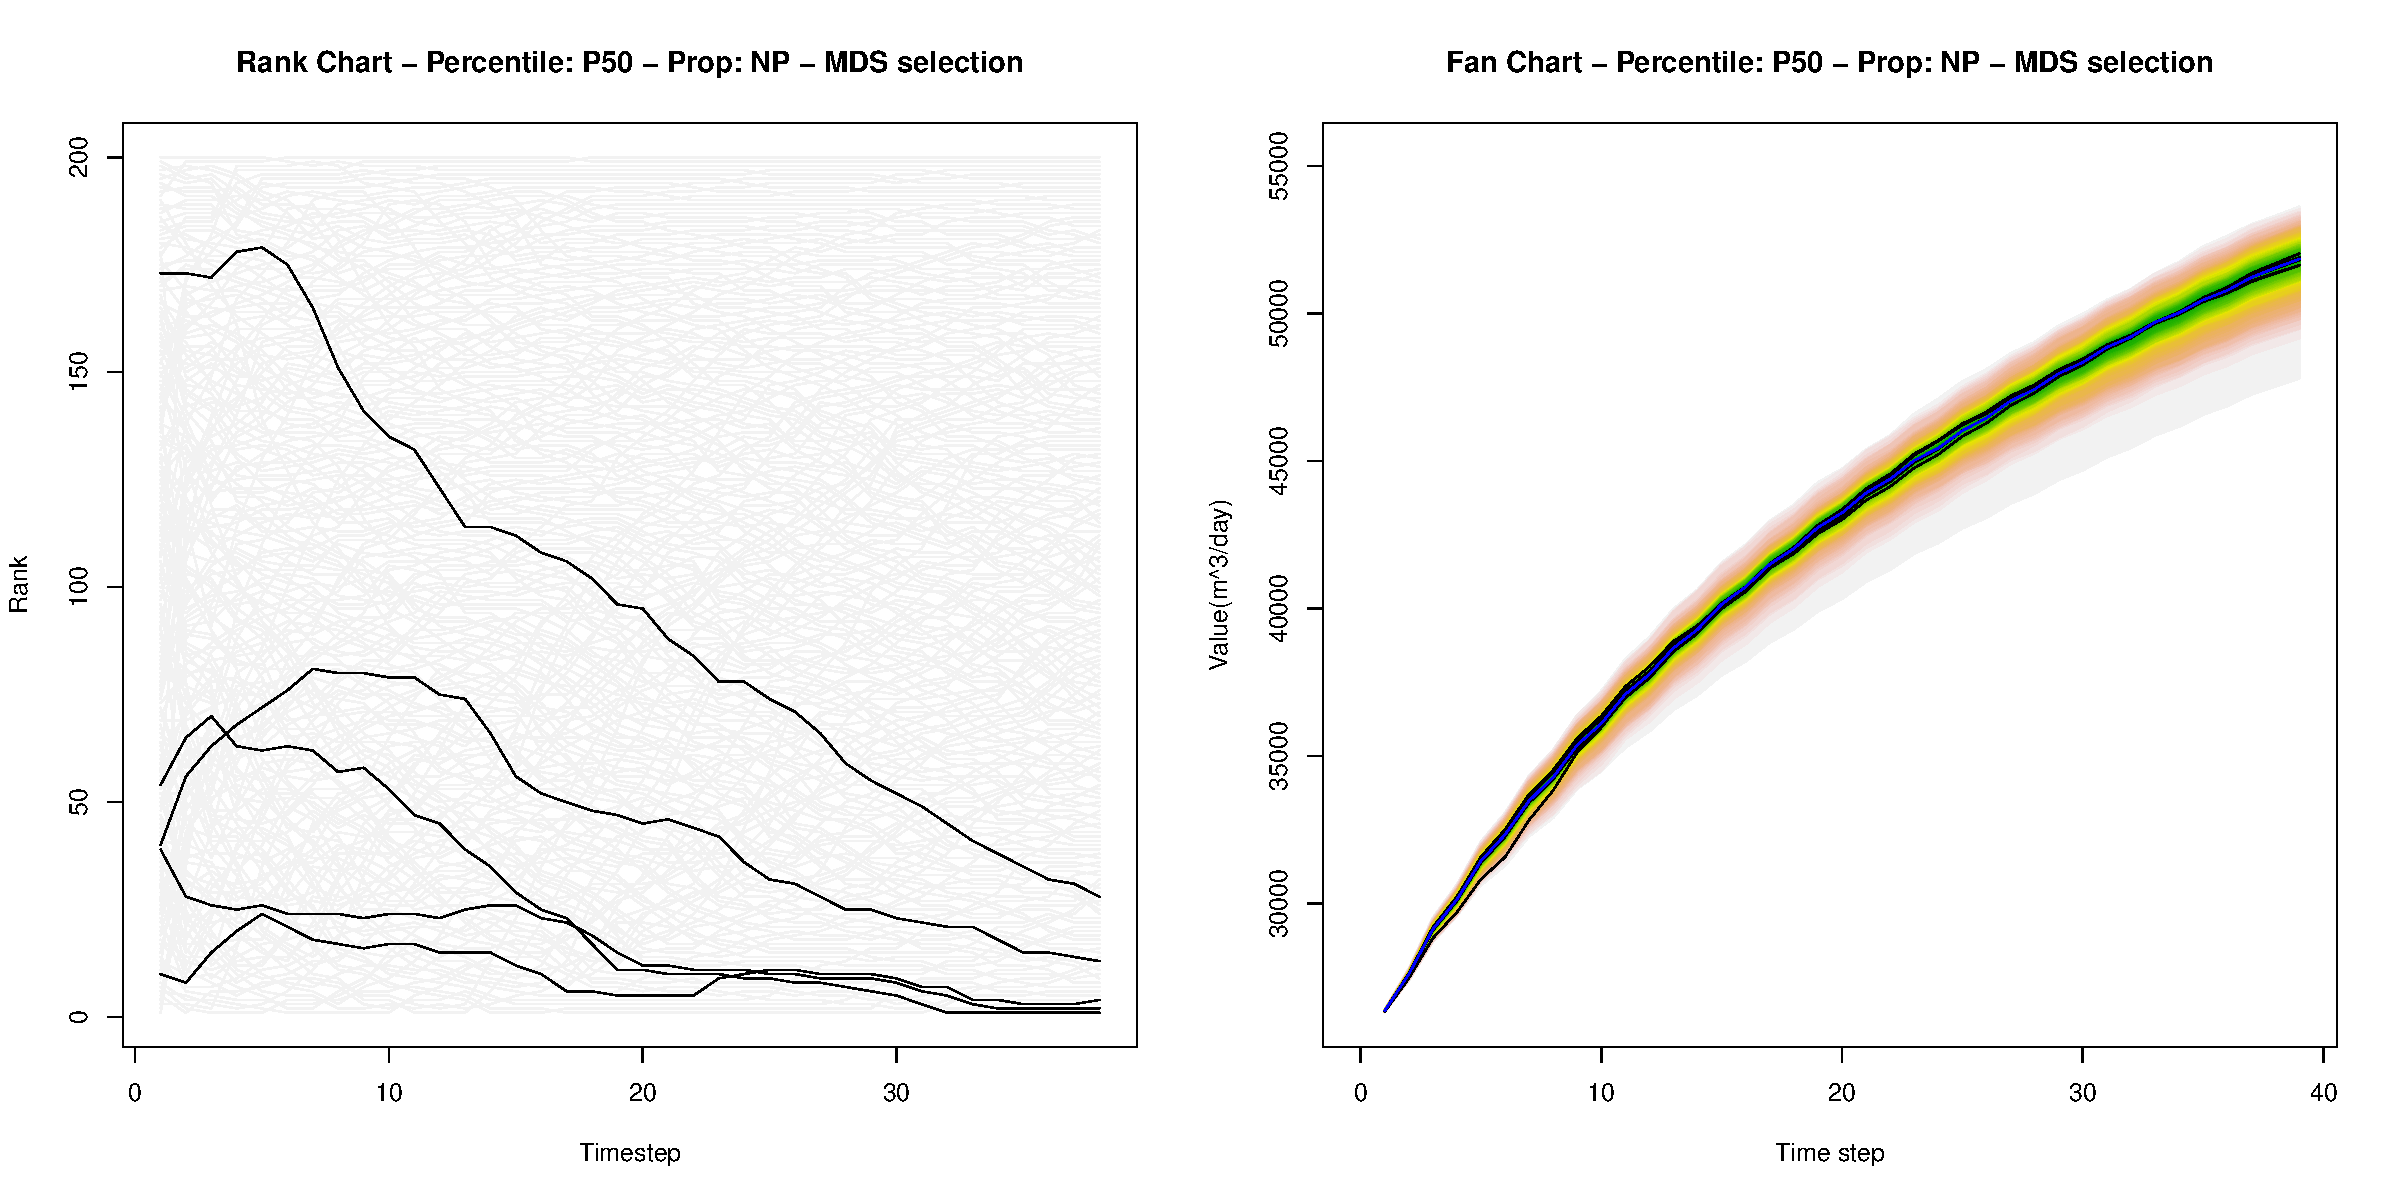
\includegraphics[width=0.9\columnwidth]{rank-fan-mds-sel-p50.pdf}
    \caption{Side-by-side rank and fan charts of the MDS projection selected curves. The selected models are UNISIM\_45, UNISIM\_69, UNISIM\_194, UNISIM\_112 and UNISIM\_110.}
    \label{fig:rank-fan-mds}
  \end{figure}
\end{frame}

\begin{frame}{MDS kNN Selection (P$_{90}$)}
  \begin{figure}[H]
    \centering
    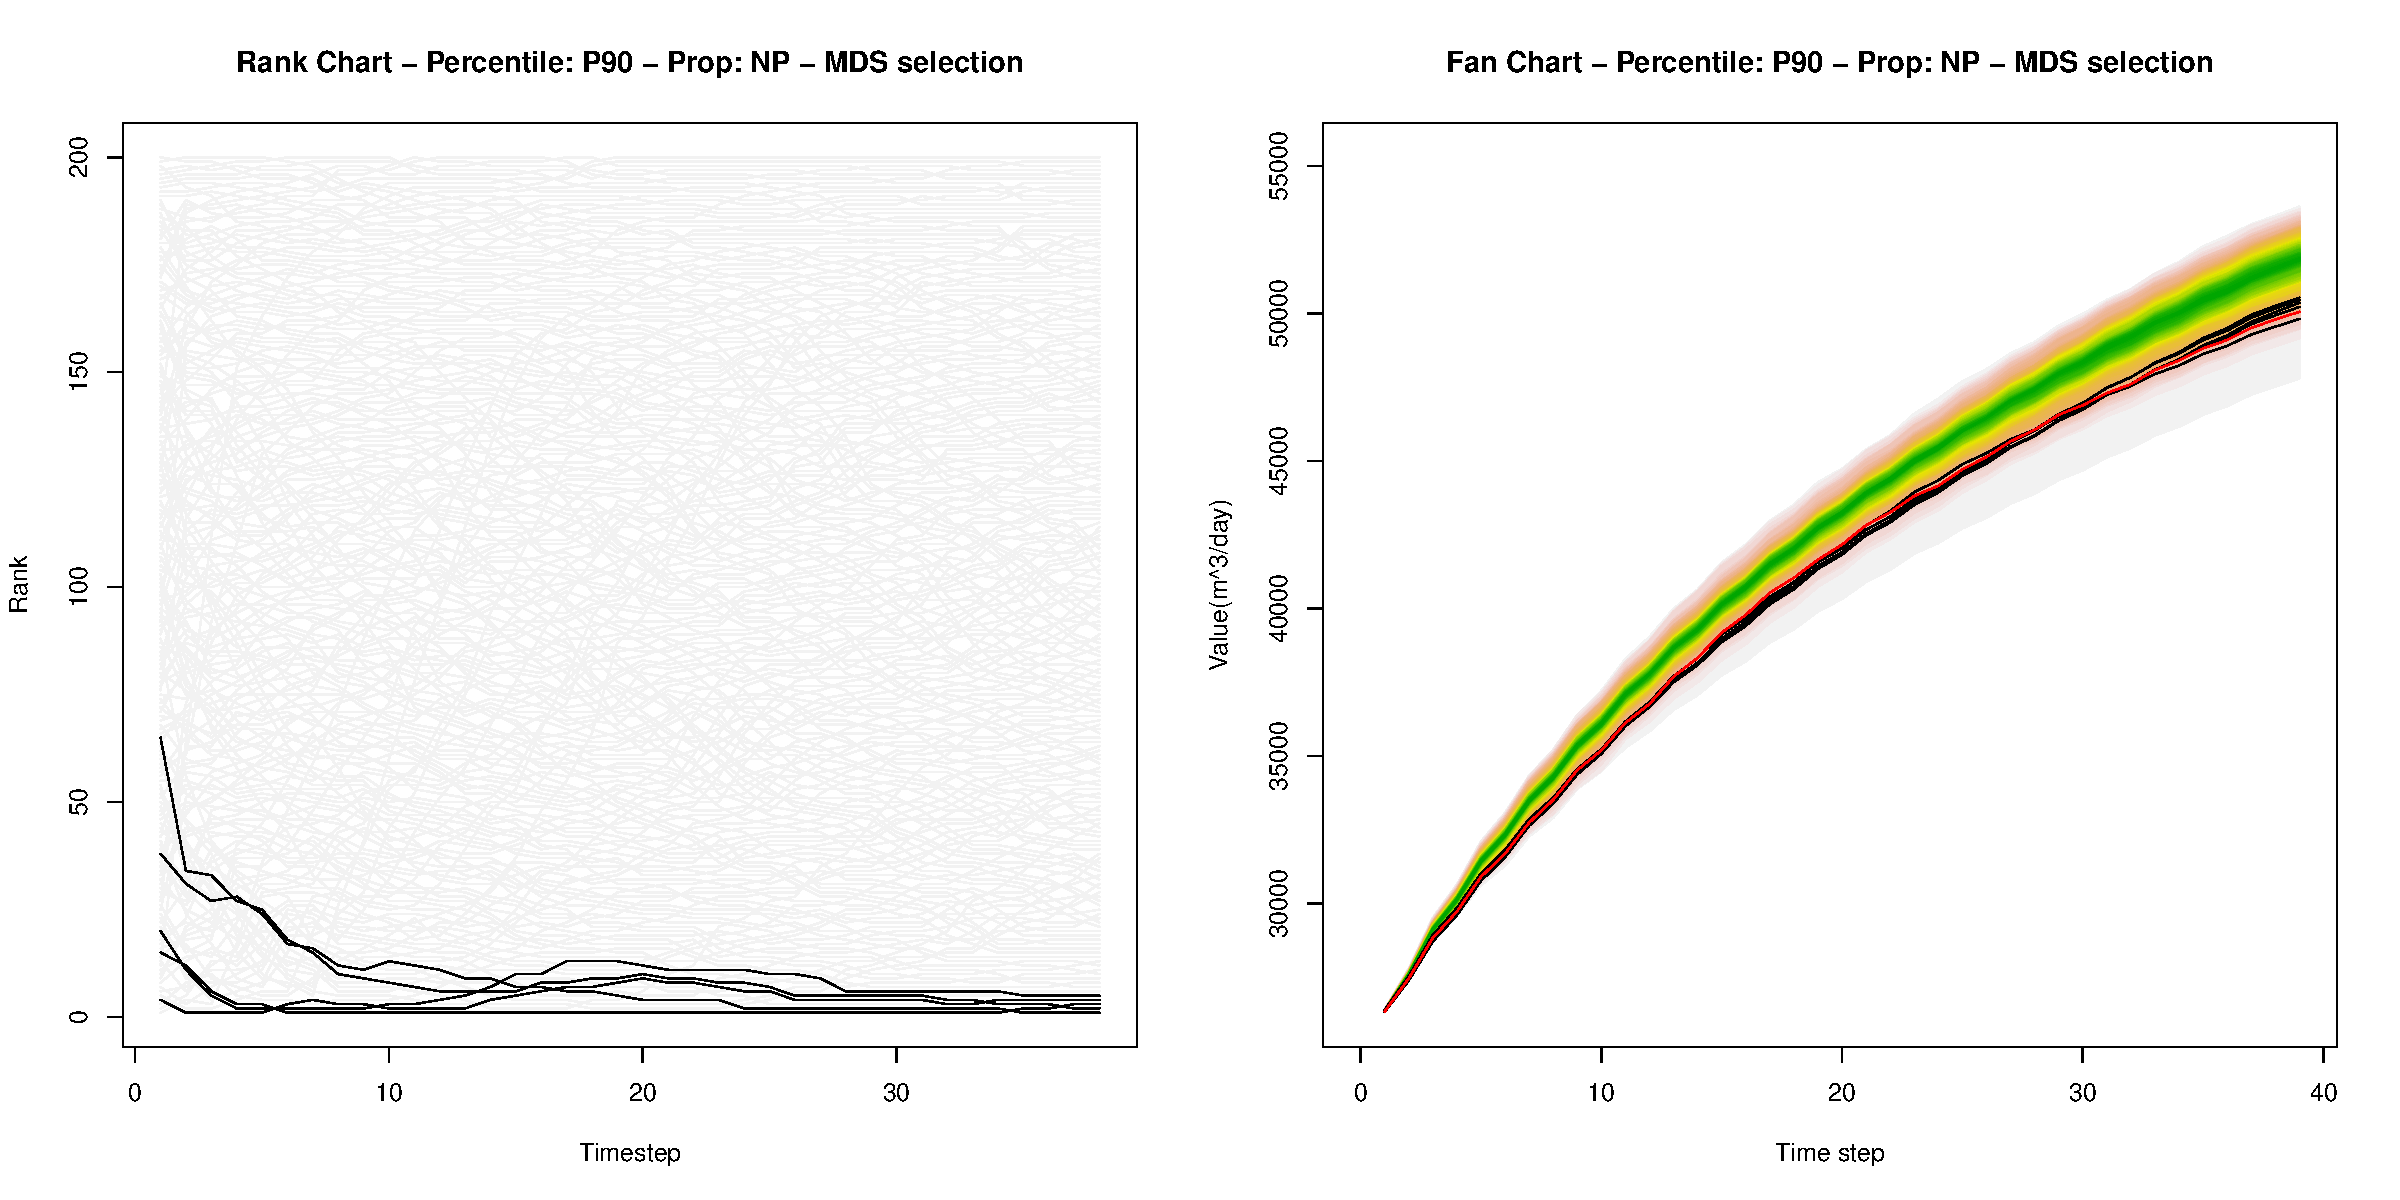
\includegraphics[width=0.9\columnwidth]{rank-fan-mds-sel-p90.pdf}
    \caption{Side-by-side rank and fan charts of the MDS projection selected curves. The selected models are UNISIM\_186, UNISIM\_73, UNISIM\_58, UNISIM\_147 and UNISIM\_53.}
    \label{fig:rank-fan-mds}
  \end{figure}
\end{frame}

\subsection{Case Study Results}
\begin{frame}{Case Study Results}
  \begin{itemize}
    \item For the P$_{10}$ and P$_{90}$ cases, the three approaches selected several models in common;
    \item For the P$_{50}$ case, only the UNISIM\_45 model was selected by the three approaches;
    \item The MDS selection found models with the poorest ranking in the P$_{50}$ case, indicating that selecting the models by the smalles distance may not be a suitable approach;
    \item The score-based and brushing \& linking approaches selected models with good overall adherence to the reference percentiles. This is also true for the MDS selection, with the exception of the P$_{50}$ case.
  \end{itemize}
\end{frame}

\section{Discussion}
\begin{frame}
  \tableofcontents[currentsection]
\end{frame}

\begin{frame}{Discussion}
  \begin{itemize}
    \item Our main motivation was that the other approaches used only the latest production values;
    \item Our hypothesis is that this may lead to a poorer selection due to the disregard for the evolution of the models;
    \item As an example, we calculated the percentiles using only the latest oil production values and selected the models closest to them as representatives;
  \end{itemize}
\end{frame}

\subsection{Empirical percentiles selection}
\begin{frame}{Empirical percentiles selection}
  \begin{figure}[H]
    \centering
    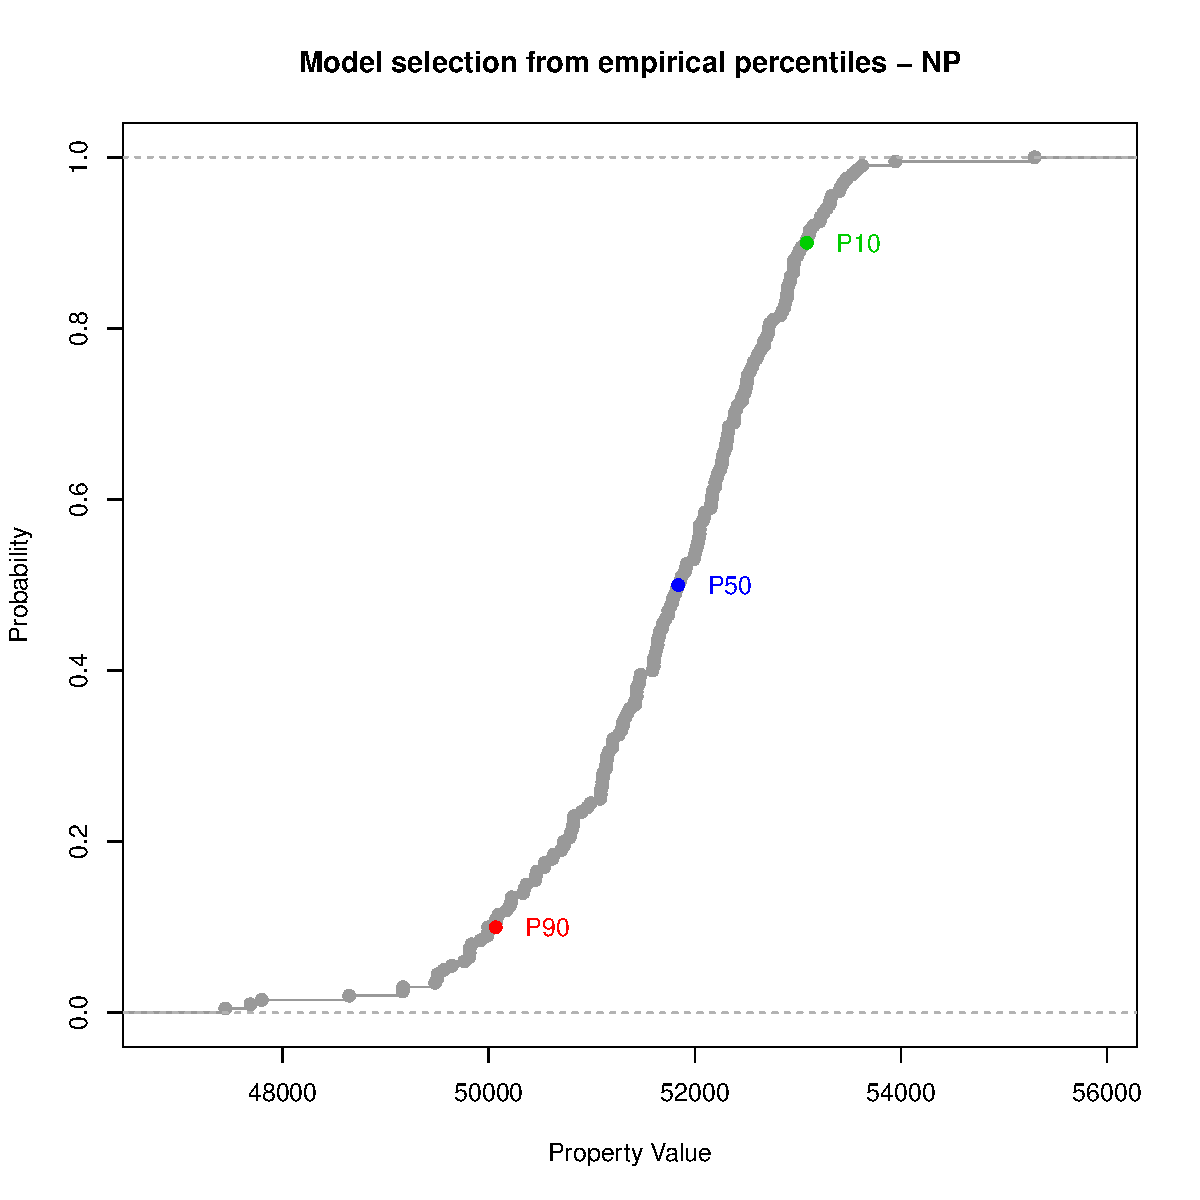
\includegraphics[width=0.48\columnwidth]{ecdf-NP.pdf}
    \caption{Empirical cumulative probability distribution of the latest production values of the cumulative oil production of UNISIM-I-H. The P$_{10}$, P$_{50}$ and P$_{90}$ models are marked in green, blue and red and correspond to the models UNISIM\_96, UNISIM\_4 and UNISIM\_172 respectively.}
    \label{fig:ecdf-NP}
  \end{figure}
\end{frame}

\begin{frame}{Empirical percentiles selection (Rank and Fan charts P$_{10}$)}
  \begin{figure}[H]
    \centering
    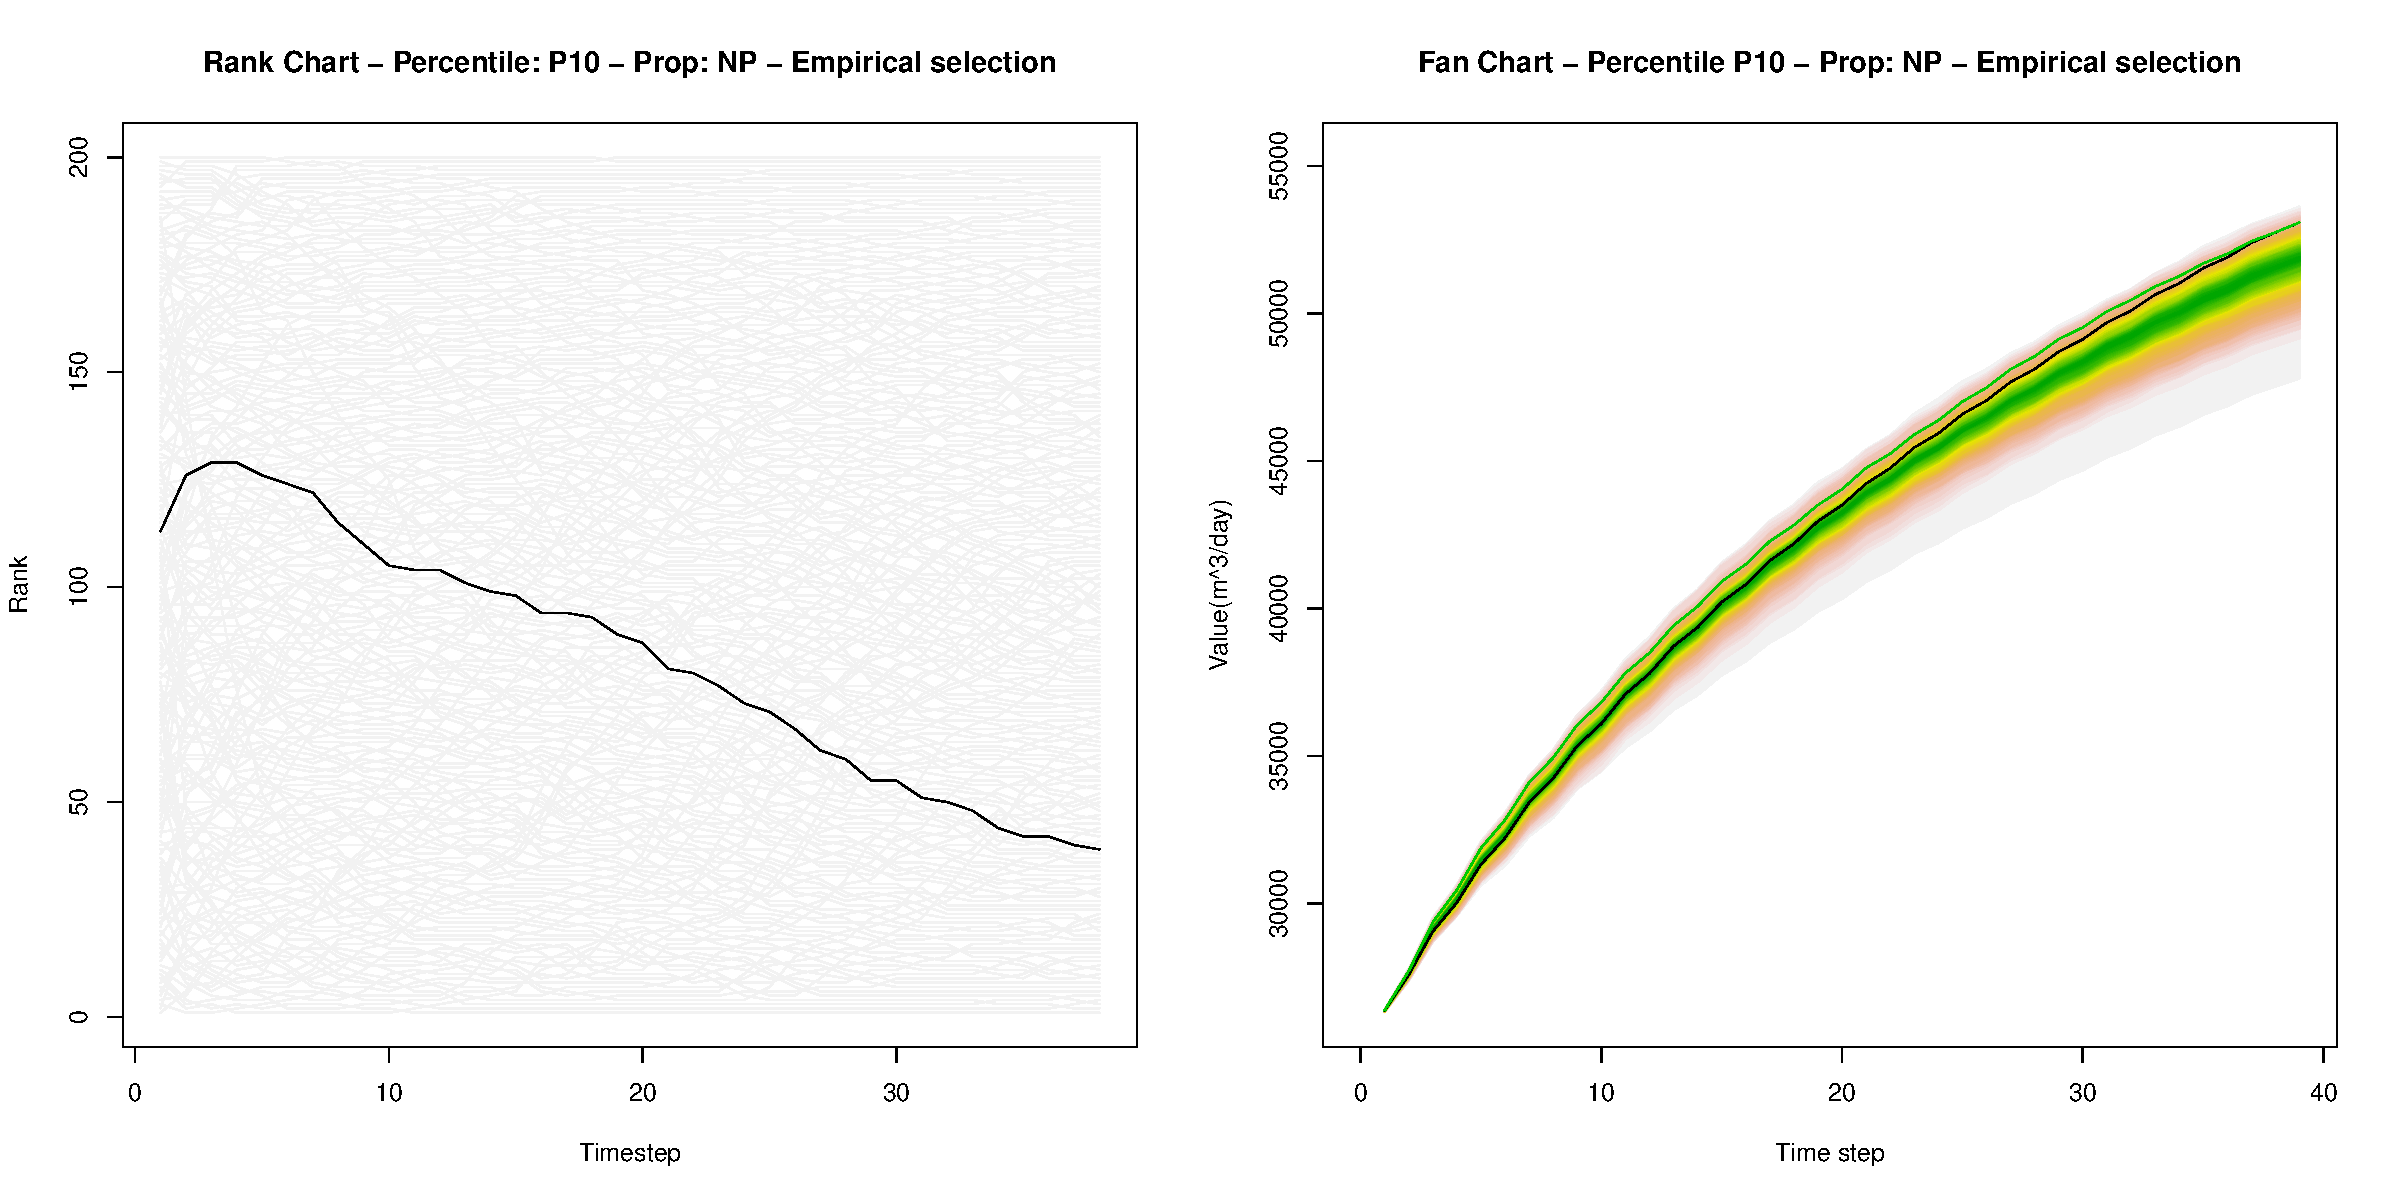
\includegraphics[width=0.9\columnwidth]{rank-fan-ecdf-p10.pdf}
    \caption{Side-by-side rank and fan charts of the models selected using the cumulative probability distribution of the latest production values.}
    \label{fig:rank-fan-ecdf}
  \end{figure}
\end{frame}

\begin{frame}{Empirical percentiles selection (Rank and Fan charts P$_{50}$)}
  \begin{figure}[H]
    \centering
    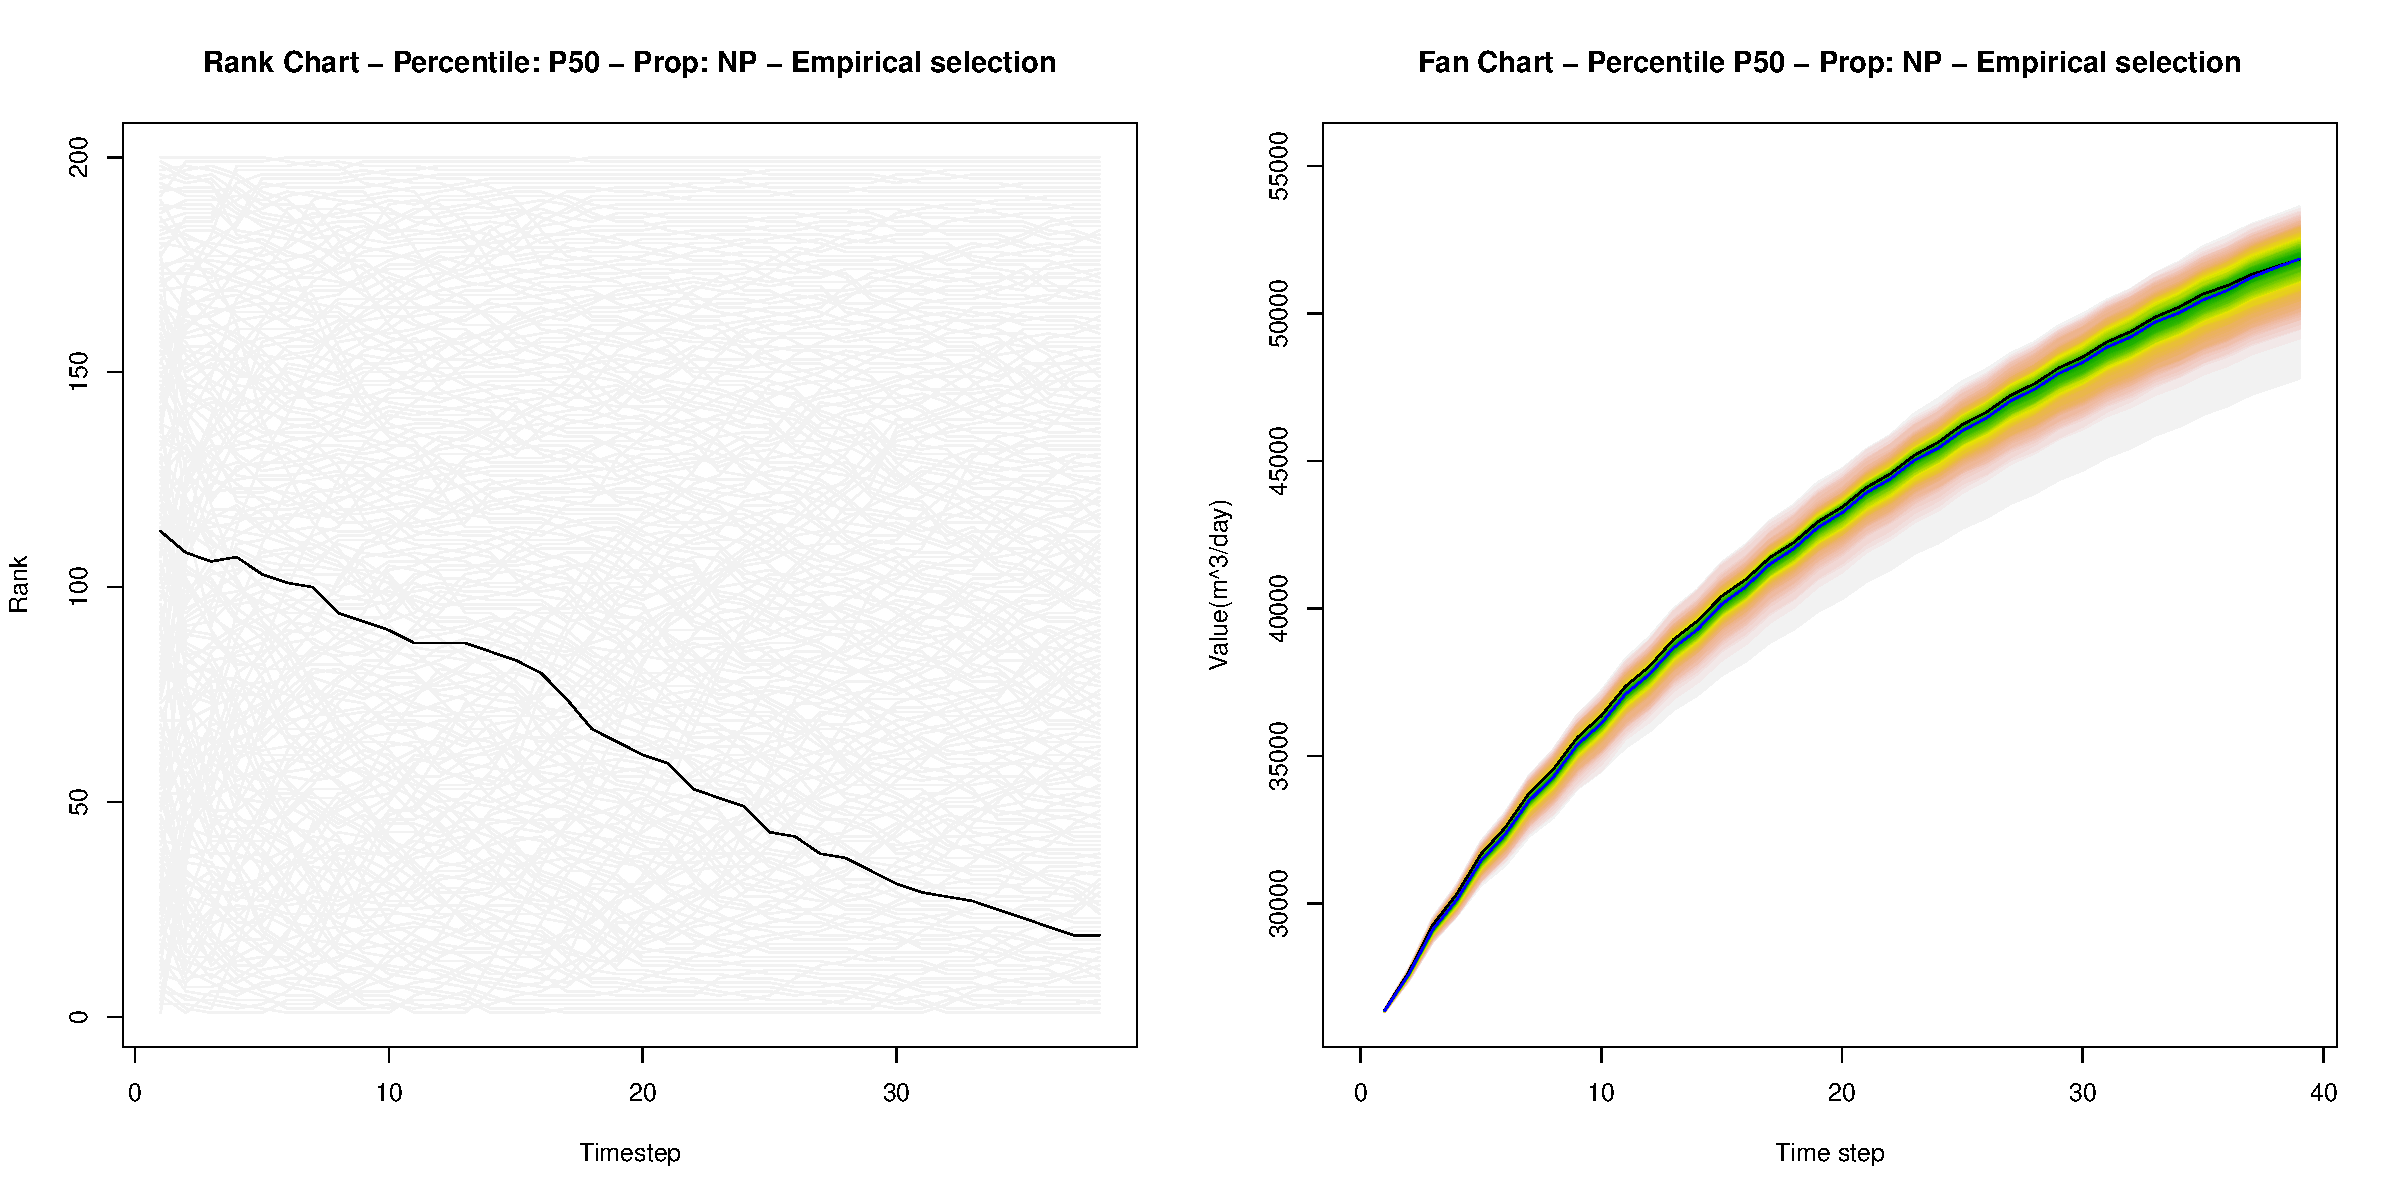
\includegraphics[width=0.9\columnwidth]{rank-fan-ecdf-p50.pdf}
    \caption{Side-by-side rank and fan charts of the models selected using the cumulative probability distribution of the latest production values.}
    \label{fig:rank-fan-ecdf}
  \end{figure}
\end{frame}

\begin{frame}{Empirical percentiles selection (Rank and Fan charts P$_{90}$)}
  \begin{figure}[H]
    \centering
    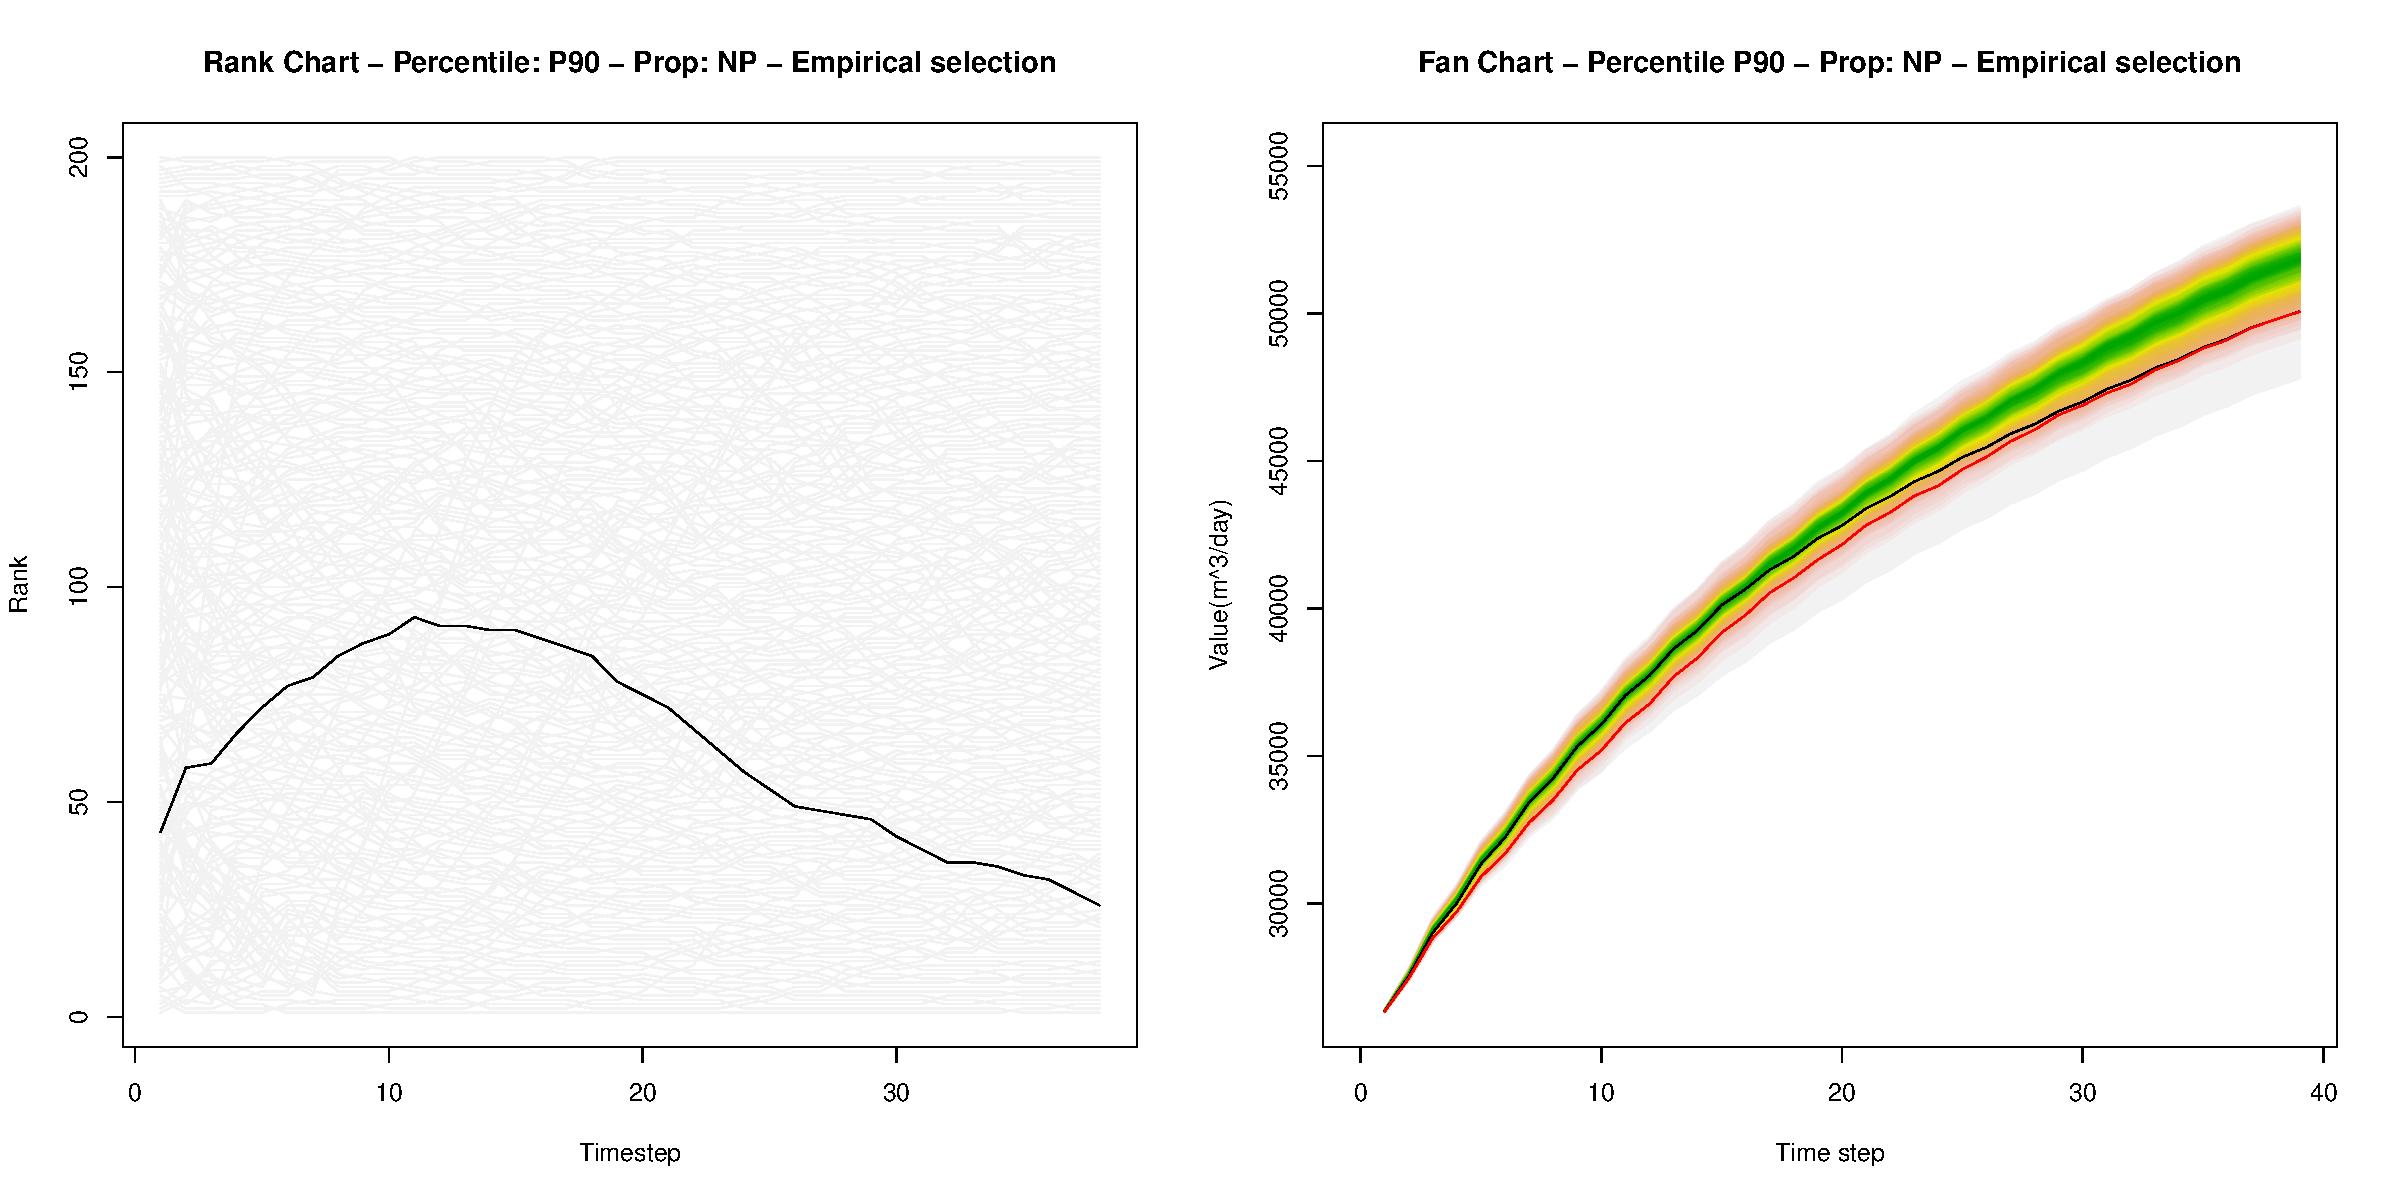
\includegraphics[width=0.9\columnwidth]{rank-fan-ecdf-p90.pdf}
    \caption{Side-by-side rank and fan charts of the models selected using the cumulative probability distribution of the latest production values.}
    \label{fig:rank-fan-ecdf}
  \end{figure}
\end{frame}

\begin{frame}{Empirical percentiles selection (MDS projection)}
  \begin{figure}[H]
    \centering
    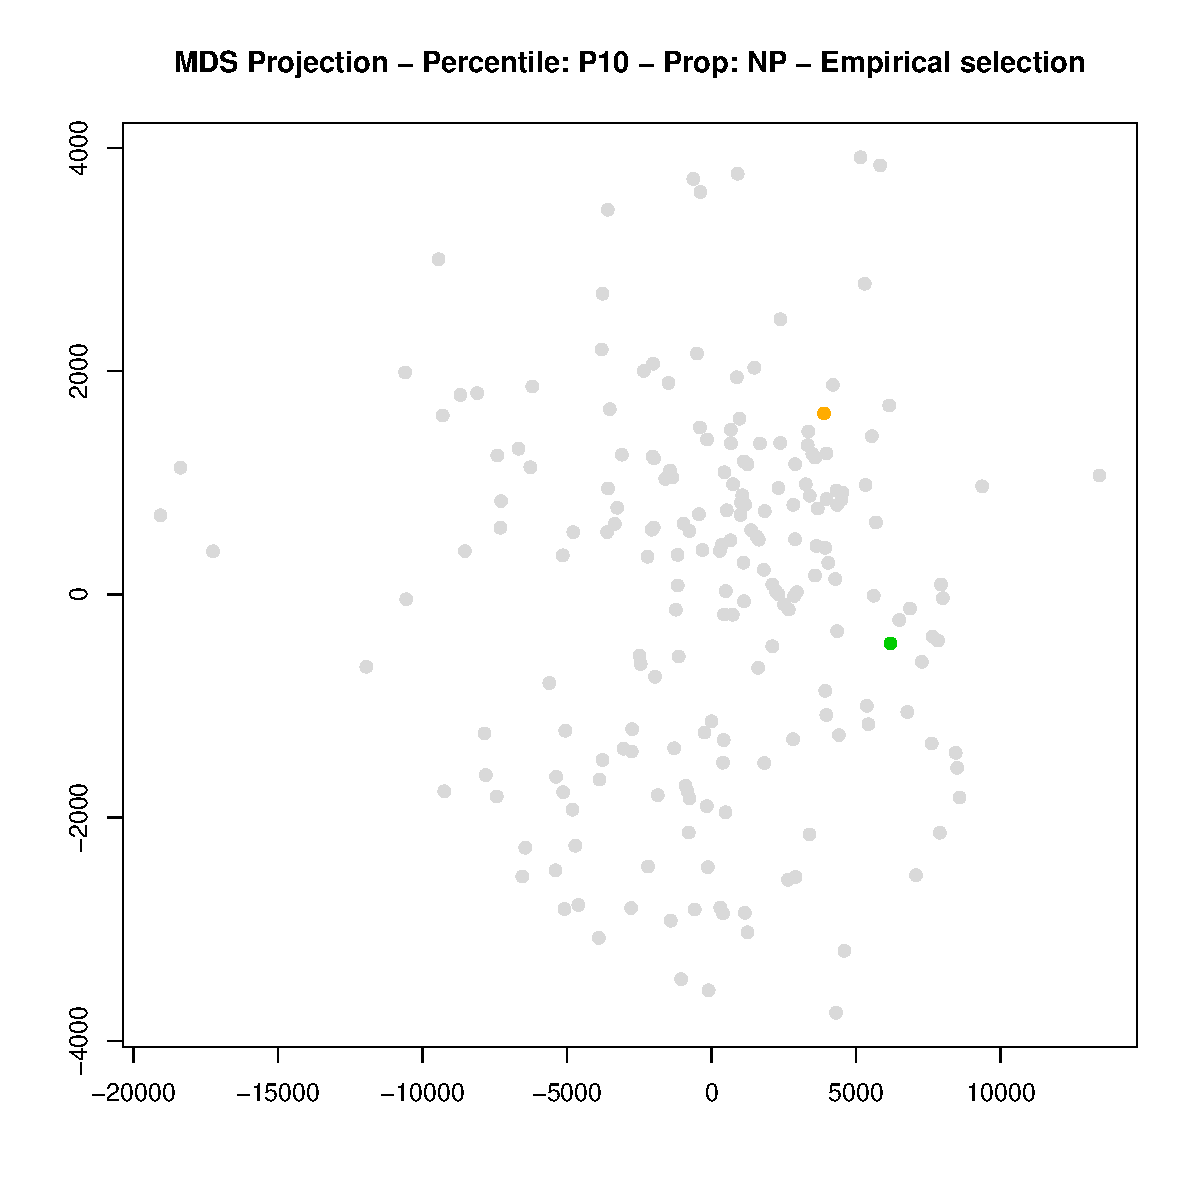
\includegraphics[width=0.33\columnwidth]{mds-ecdf-NP-p10.pdf}
    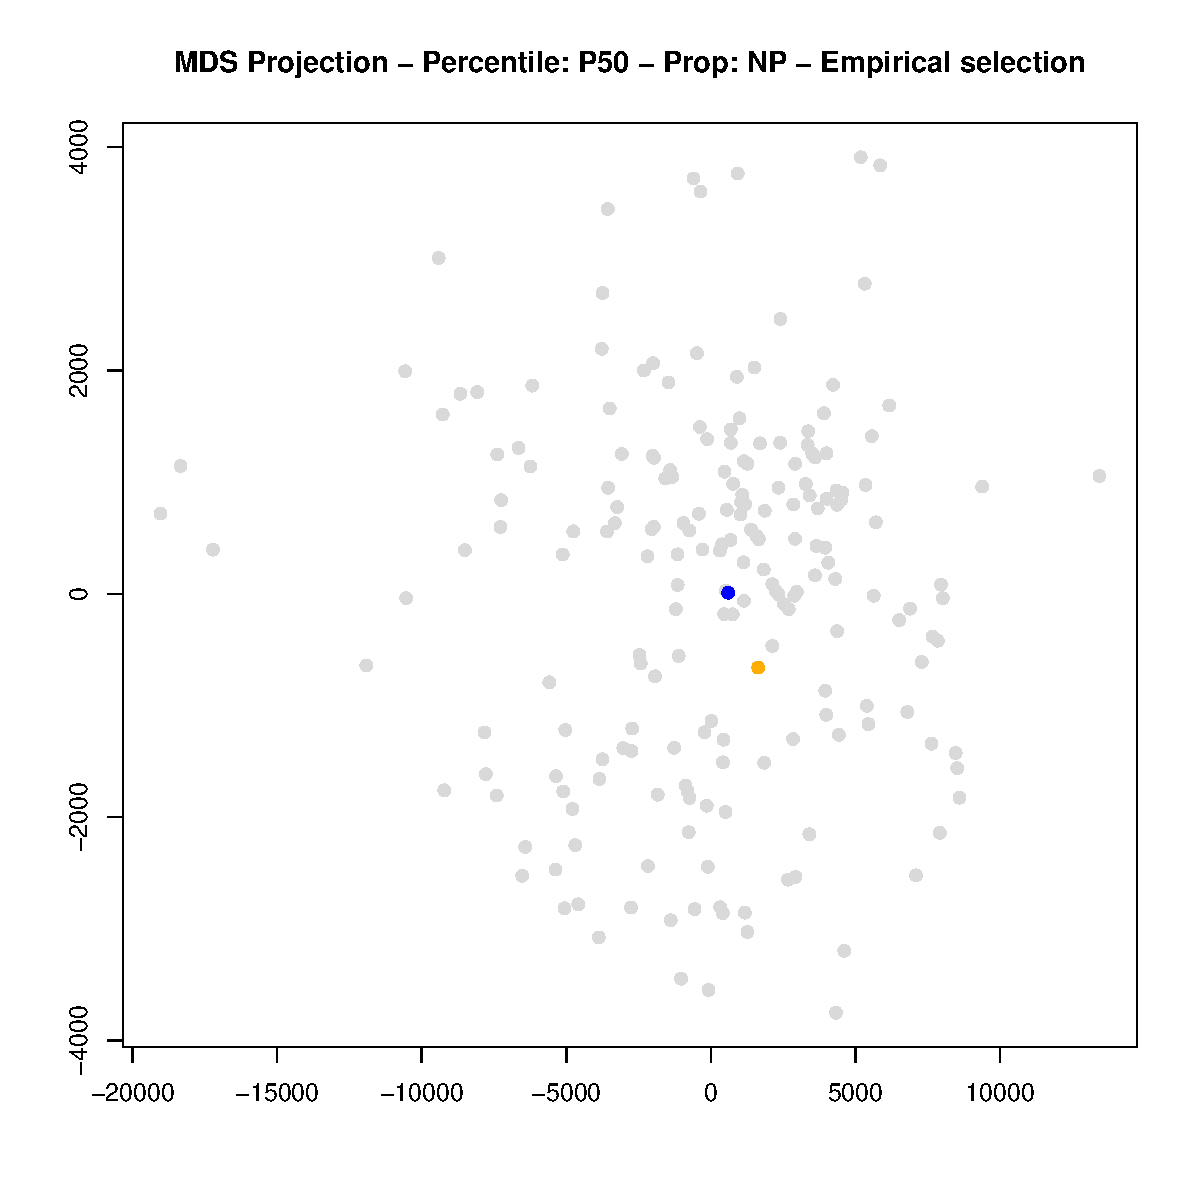
\includegraphics[width=0.33\columnwidth]{mds-ecdf-NP-p50.pdf}
    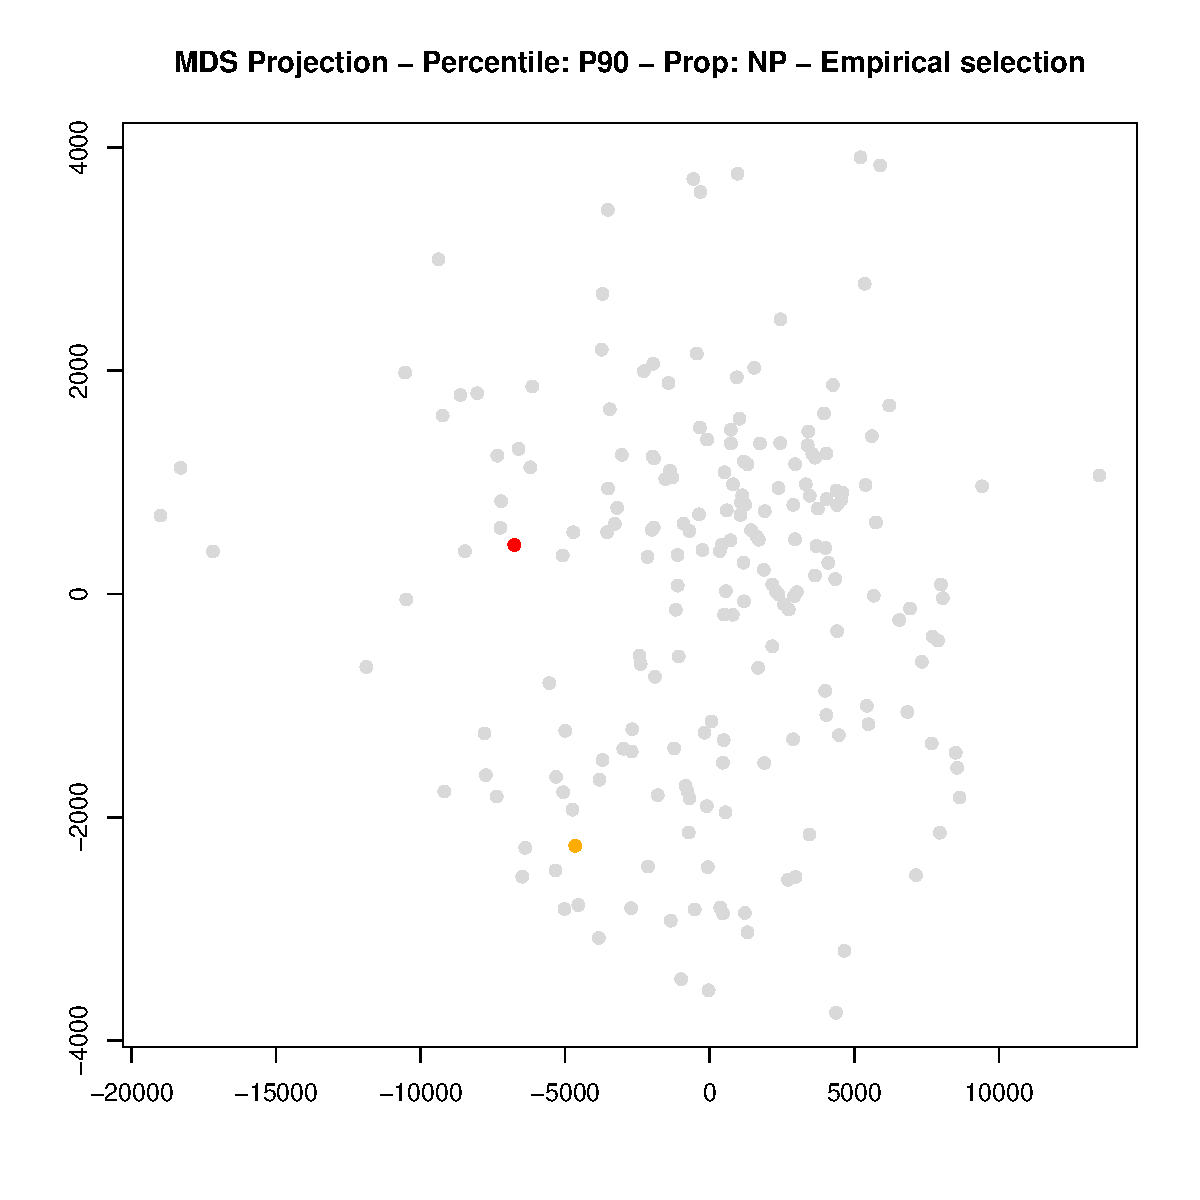
\includegraphics[width=0.33\columnwidth]{mds-ecdf-NP-p90.pdf}
    \caption{MDS projections of the ensemble elements with the selected entities in orange and the P$_{10}$, P$_{50}$ and P$_{90}$ models in green, blue and red respectively.}
    \label{fig:mds-ecdf}
  \end{figure}
\end{frame}

\begin{frame}{Discussion}
  \begin{itemize}
    \item The models selected by using only the latest production values do not fit the percentiles well;
    \item Their ranking is poor during the whole simulation time;
    \item The model projections are located far from the projected percentiles;
  \end{itemize}
\end{frame}

\section{Conclusions}
\begin{frame}
  \tableofcontents[currentsection]
\end{frame}

\begin{frame}{Conclusions}
  \begin{itemize}
    \item Development of the Rank Chart as a graphical tool to analyze the adherence of time series to a reference curve;
    \item Development of a score-based approach to automatically select a subset of possible representative elements;
    \item Analysis of the whole range may lead to a better selection;
    \begin{itemize}
      \item Use of one property may lead to the selection of sub-optimal models when compared to other approaches \footfullcite{selection-sarma:2013} \footfullcite{meira:2016}.
    \end{itemize}
  \end{itemize}
\end{frame}

\subsection{Future Work}
\begin{frame}{Future Work}
  \begin{itemize}
    \item Validate our method with expert users;
    \item Look for ways to include multiple properties to select models that are representative in several aspects;
    \item Adapt the rank chart (if possible) to represent multivariate time series;
    \item Adapt the score selection to use pre simulation parameters.
  \end{itemize}
\end{frame}

\section{}
\begin{frame}
  \titlepage
\end{frame}

\end{document}
